\documentclass{PoS}
\usepackage{xspace}
\usepackage{subcaption}

\title{Measurements of Vector boson fusion with the ATLAS detector}

\ShortTitle{Measurements of Vector boson fusion with the ATLAS detector}

\author{\speaker{Kurt Brendlinger},
        on behalf of the ATLAS Collaboration\\
%%         \thanks{A footnote may follow.}\\
       Deutsches Elektronen-Synchrotron (DE)\\
       E-mail: \email{kurt.brendlinger@cern.ch}}

%\author{Another Author\\
%        Affiliation\\
%        E-mail: \email{...}}

\def\wjj{\ensuremath{W\kern -0.2em j\kern -0.1emj}\xspace}
\def\zjj{\ensuremath{Z\kern -0.1em j\kern -0.1emj}\xspace}
\def\vjj{\ensuremath{V\kern -0.2em j\kern -0.1emj}\xspace}
\def\w{\ensuremath{W}\xspace}
\def\z{\ensuremath{Z}\xspace}
\def\mjj{\ensuremath{M_{jj}}}

\abstract{%The ATLAS experiment with data collected by the Large Hadron Collider (LHC).
The most recent ATLAS results on the production of single \w and \z bosons with two jets at high invariant
mass at centre-of-mass energies of 7, 8 and 13 TeV are presented. Integrated and differential cross
sections are measured in different phase space regions with varying degree of sensitivity to the
electroweak production in vector boson fusion. The cross section for the electroweak \w boson production
has been extracted for both integrated and for the first time differential distributions. In addition,
the cross-section for the electroweak production of two jets in association with a \z boson is measured
for the first time at a centre-of-mass energy of 13 TeV. The results are compared to state-of-the-art
theory predictions and are used to constrain anomalous gauge couplings.
}

\FullConference{The European Physical Society Conference on High Energy Physics\\
                 5-12 July\\
                 Venice, Italy}

\begin{document}

This talk presented stuff from the ATLAS detector \cite{Aad:2008zzm} collected by the
LHC \cite{Evans:2008zzb}.
The first result presented is a measurement of the \wjj production \cite{Aaboud:2017fye}.
The second result is a \zjj result.

Both analyses seek to isolate and measure electroweak (EW) vector boson production in association with
two jets.

Both analyses exploit the signature of EW \vjj production to separate it from QCD production modes.
First, the invariant mass of the two leading jets is typically larger in EW production than
in QCD production.
Furthermore, in EW \vjj production the vector boson is typically emitted inside the
rapidity range bounded by the two leading jets, with no jet radiation in this range due to the absence
of color connection between the incoming partons.
By contrast, in QCD production the \w boson can be emitted outside this ``jet rapidity gap,'' and
additional jets can be emitted inside the gap.
Both the \wjj and \zjj analyses restrict the vector boson decay products to be inside the jet rapidity
gap and limit the jet radiation inside the gap.

%% Both analyses use a similar approach to measure the QCD and EW components of their respective
%% signal regions. The fraction of each production mode is obtained using a fit to the \mjj spectrum

Both analyses use similar approaches to measure the QCD and EW components of their respective signal
regions.

\section{\wjj Production Measurement}

\begin{figure}[t!]
  %\centering
  \begin{subfigure}[t]{0.74\textwidth}
    \centering
    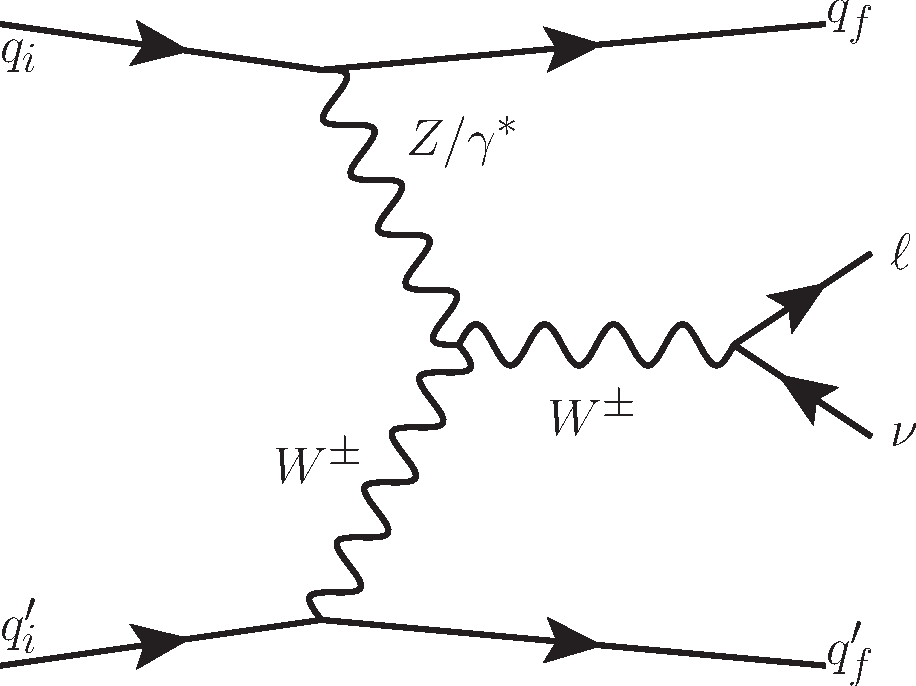
\includegraphics[width=.35\textwidth]{STDM-2014-11/fig_01a.pdf}~~
    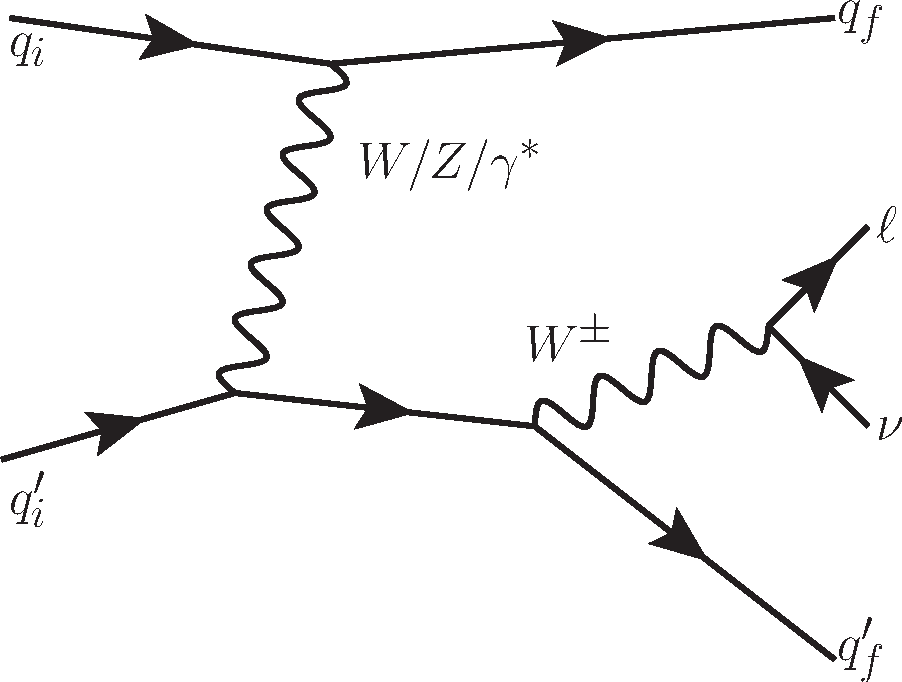
\includegraphics[width=.35\textwidth]{STDM-2014-11/fig_01b.pdf}\\ \vspace{5mm}
    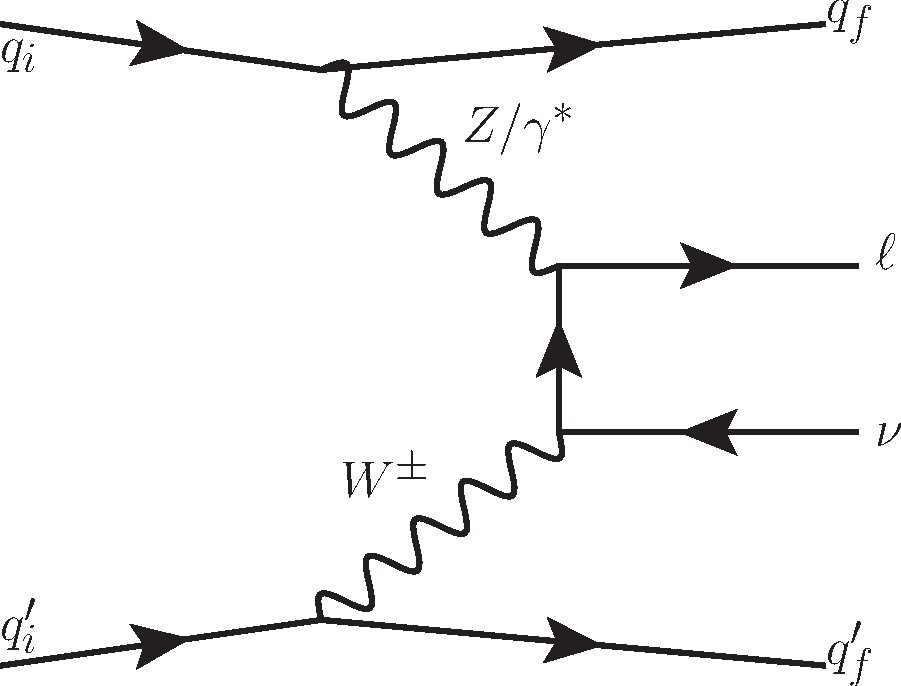
\includegraphics[width=.35\textwidth]{STDM-2014-11/fig_01c.pdf}
    \caption{}
  \end{subfigure}%
  ~
  \begin{subfigure}[t]{0.26\textwidth}
    \centering
    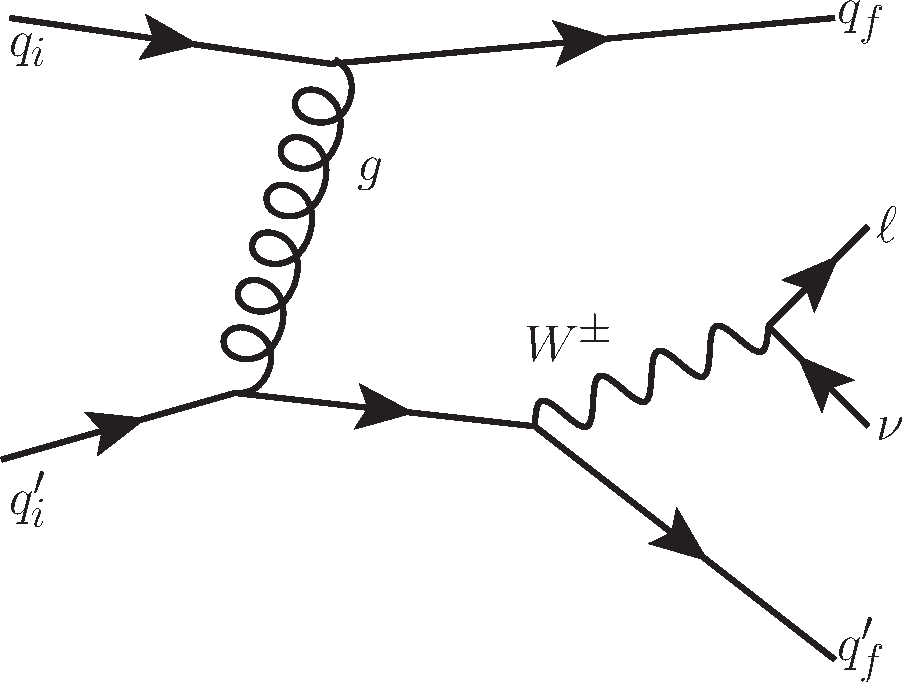
\includegraphics[width=.99\textwidth]{STDM-2014-11/fig_02a.pdf}\\ \vspace{5mm}
    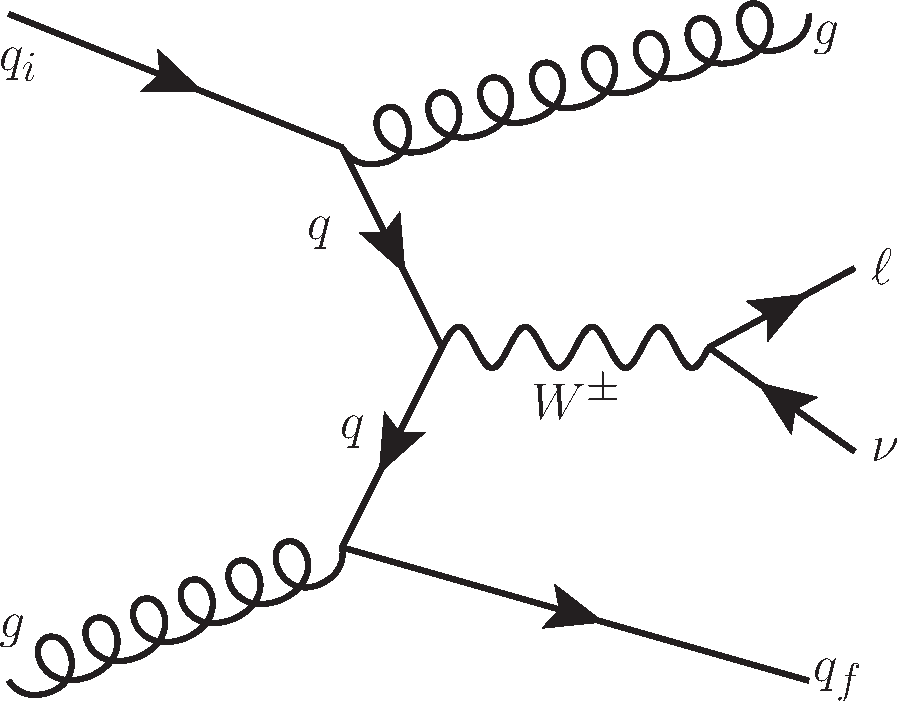
\includegraphics[width=.99\textwidth]{STDM-2014-11/fig_02b.pdf}
    \caption{}
  \end{subfigure}
  \caption{Feynman diagrams of (a) EW and (b) strong \wjj production.}
\end{figure}

Figure~\ref{wjj-cartoons}.

\begin{figure}
\centering
\raisebox{0.3\height}{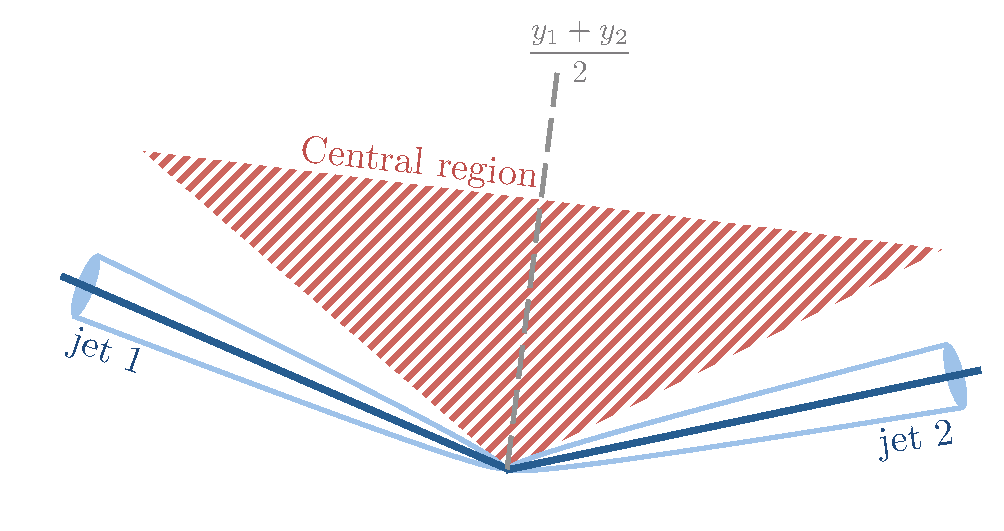
\includegraphics[width=.54\textwidth]{STDM-2014-11/fig_03.pdf}}
%% 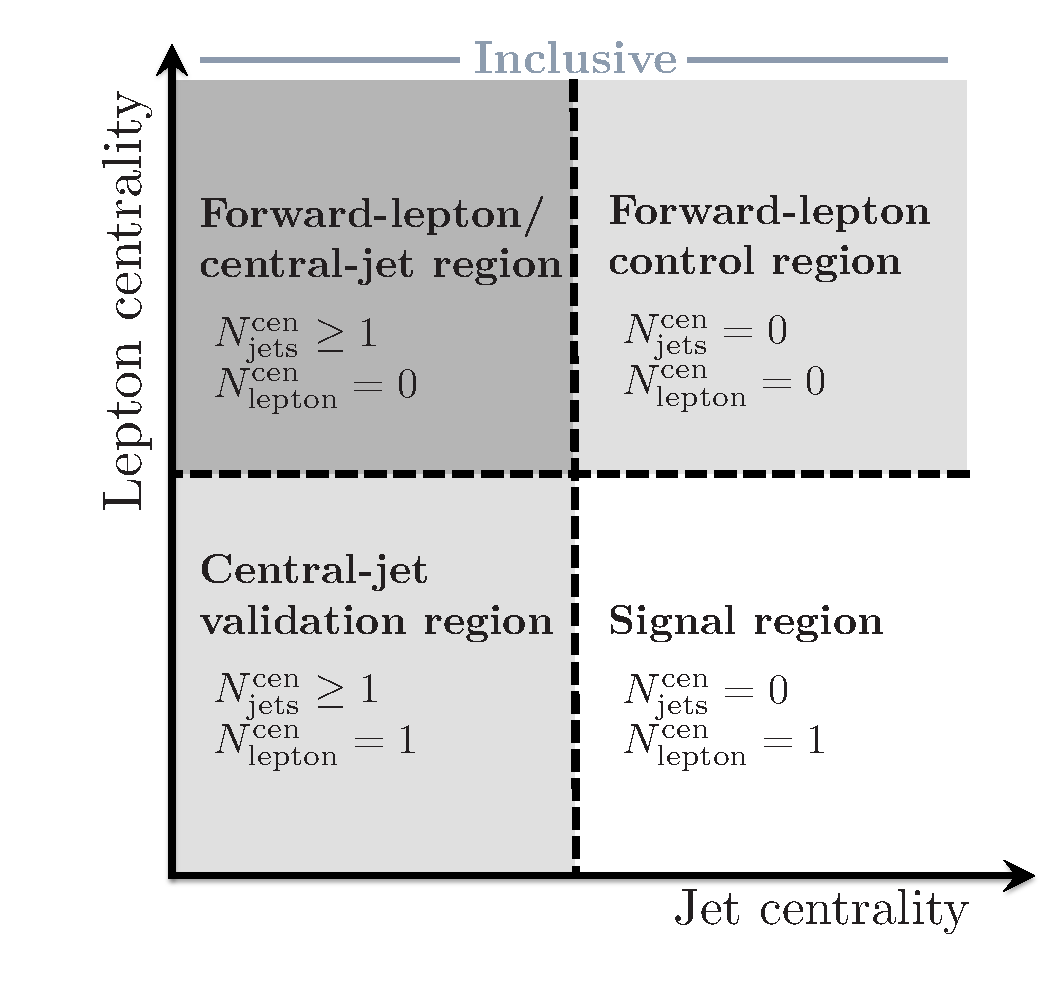
\includegraphics[width=.49\textwidth]{STDM-2014-11/fig_04.pdf}
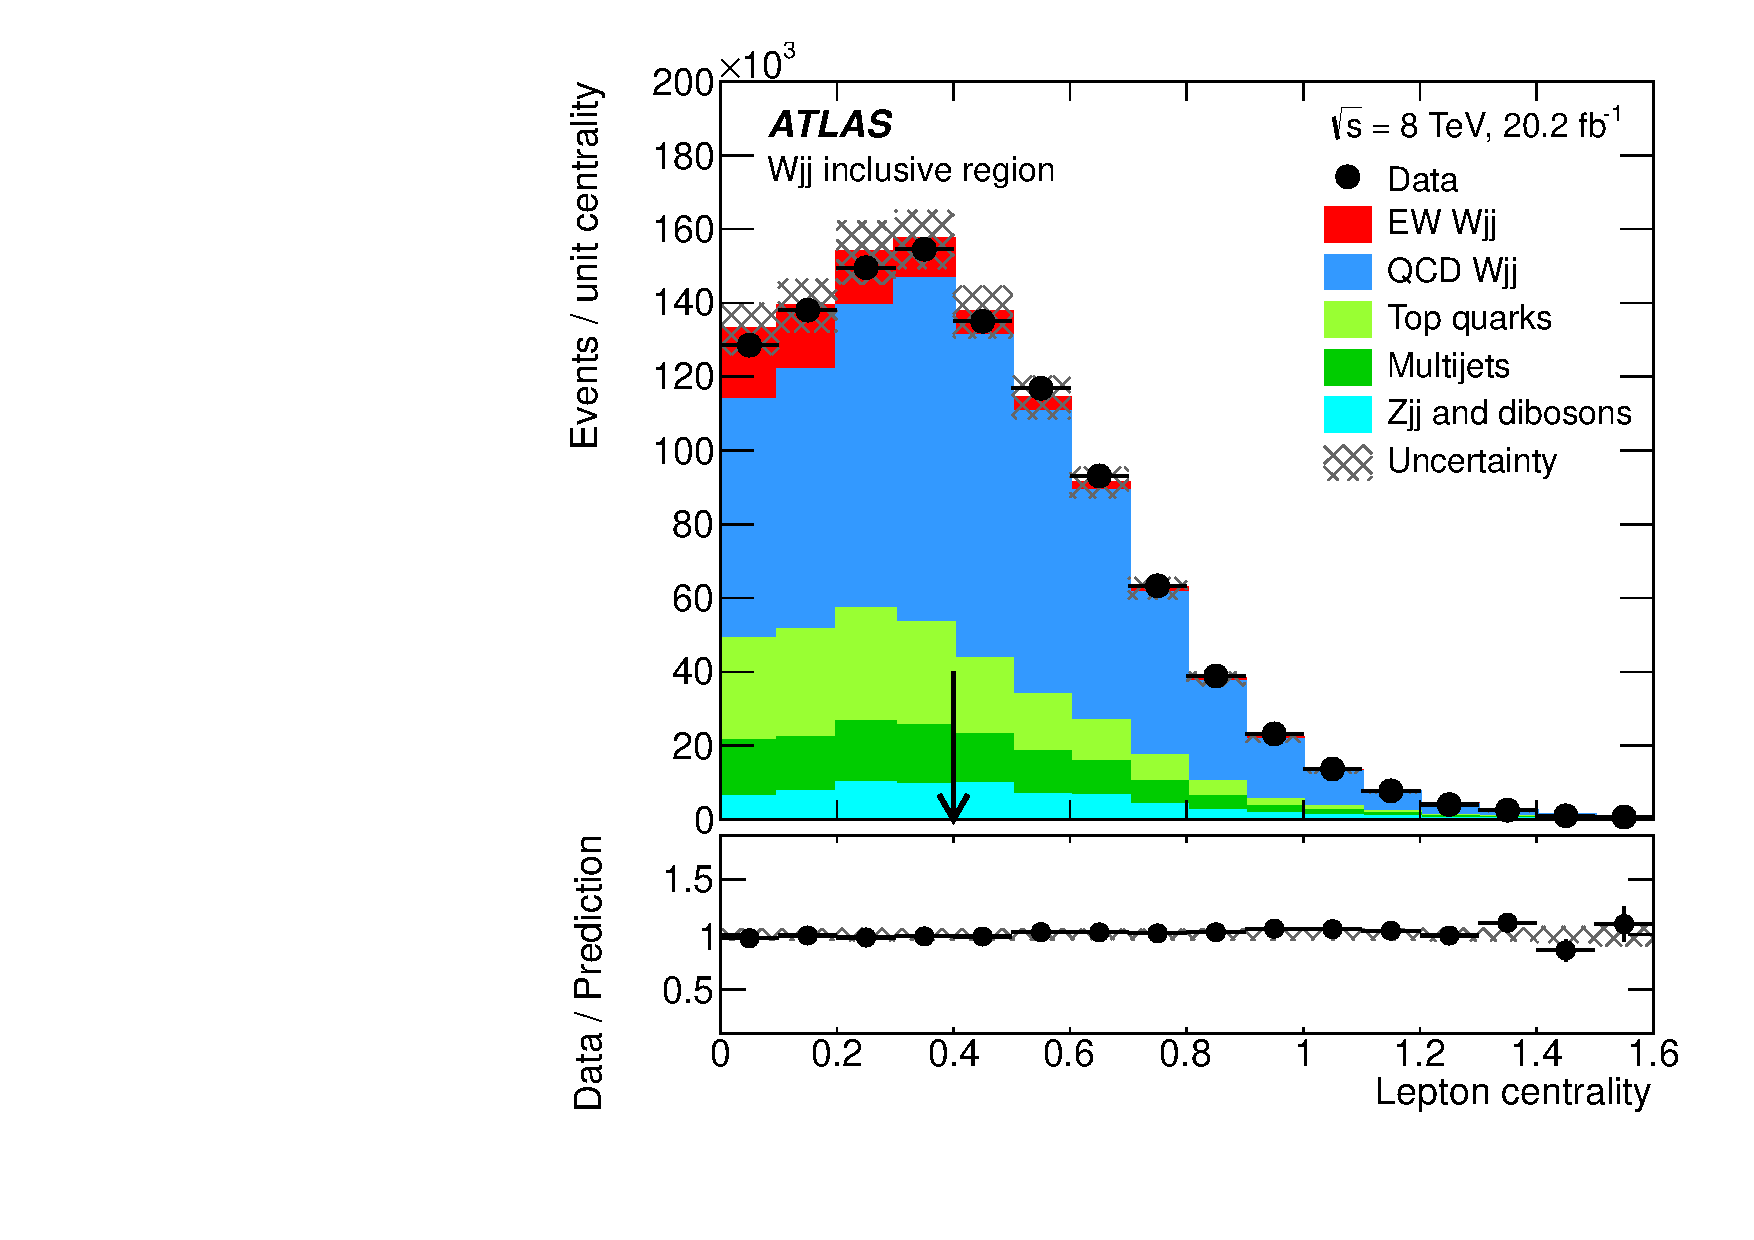
\includegraphics[width=.44\textwidth]{STDM-2014-11/fig_05b.pdf}
  \caption{Left: Depiction of...}
  \label{wjj-cartoons}
\end{figure}

%% Figure~\ref{wjj-discriminating-variables}.
%% \begin{figure}
%% \centering
%% 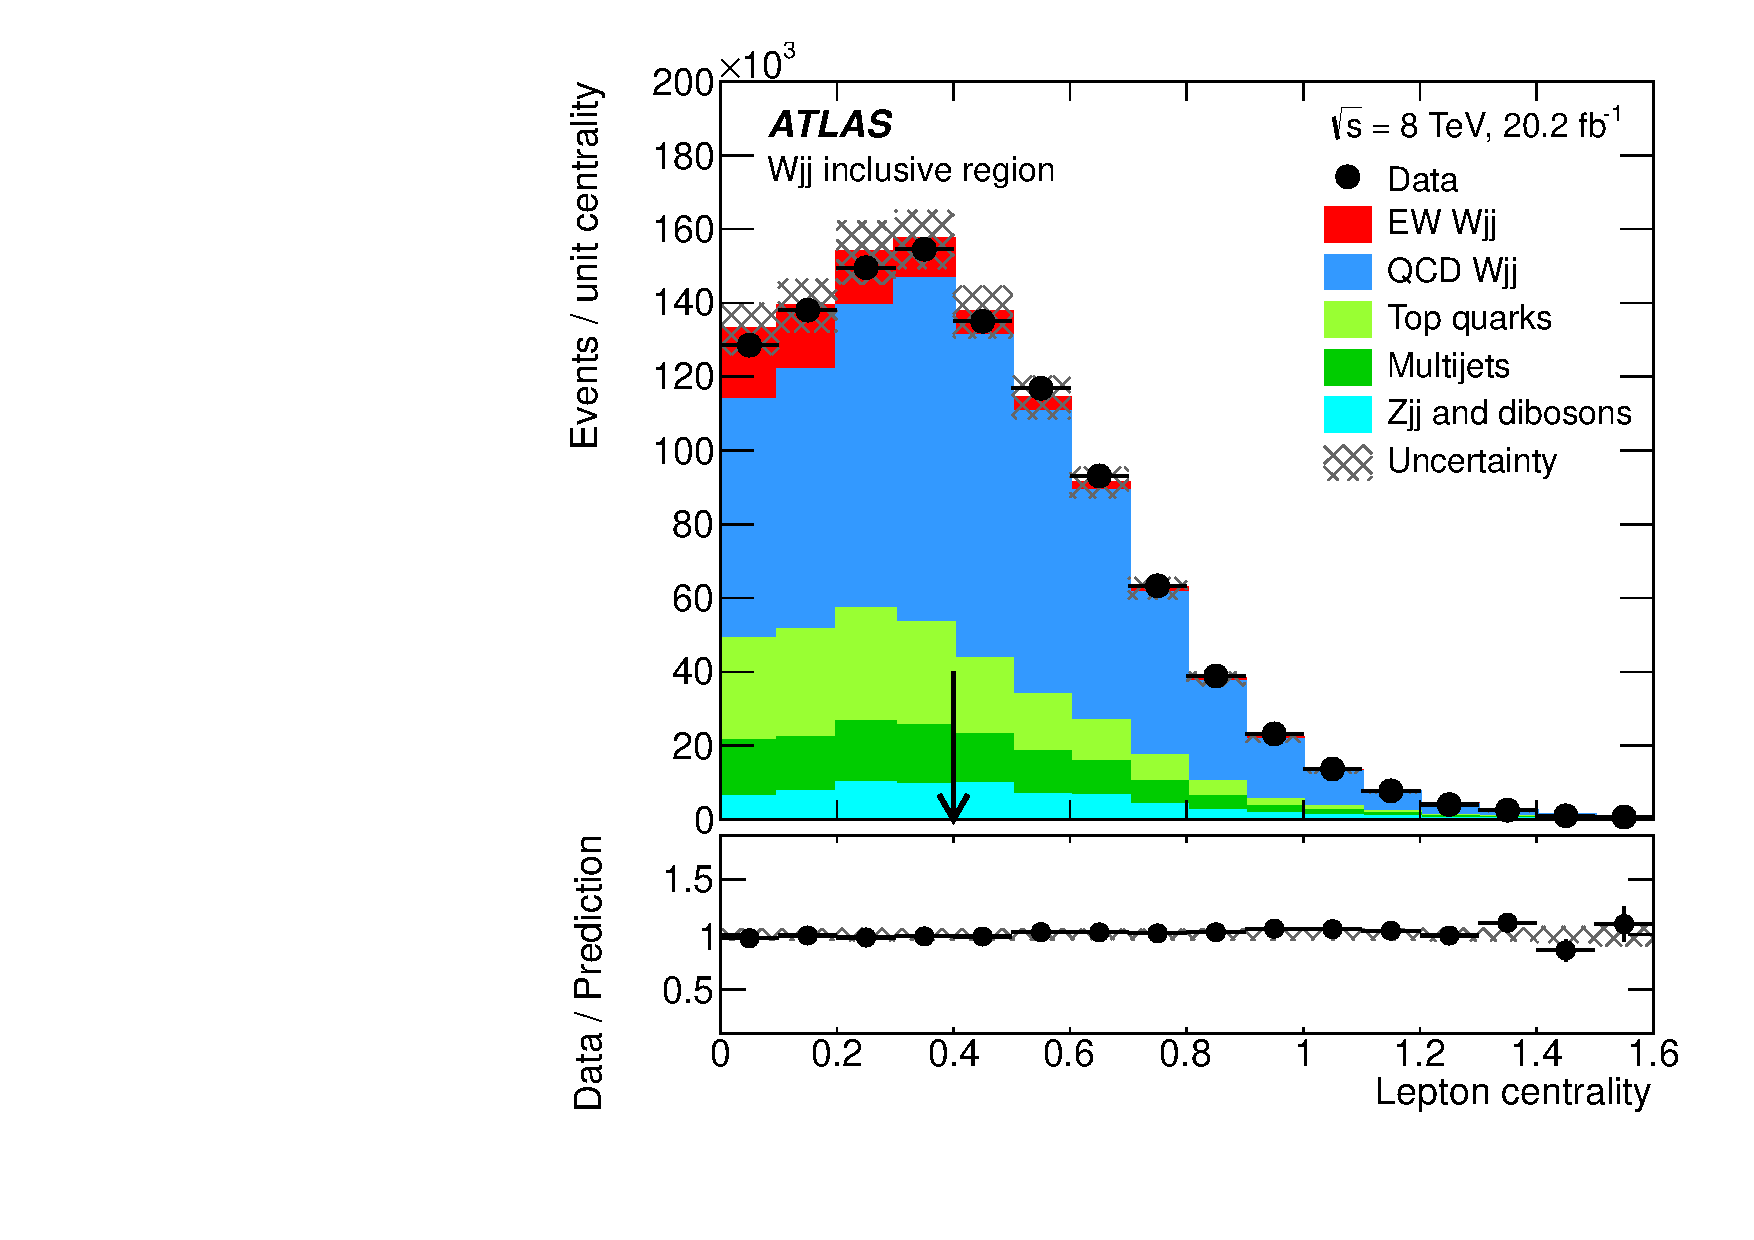
\includegraphics[width=.49\textwidth]{STDM-2014-11/fig_05b.pdf}
%% 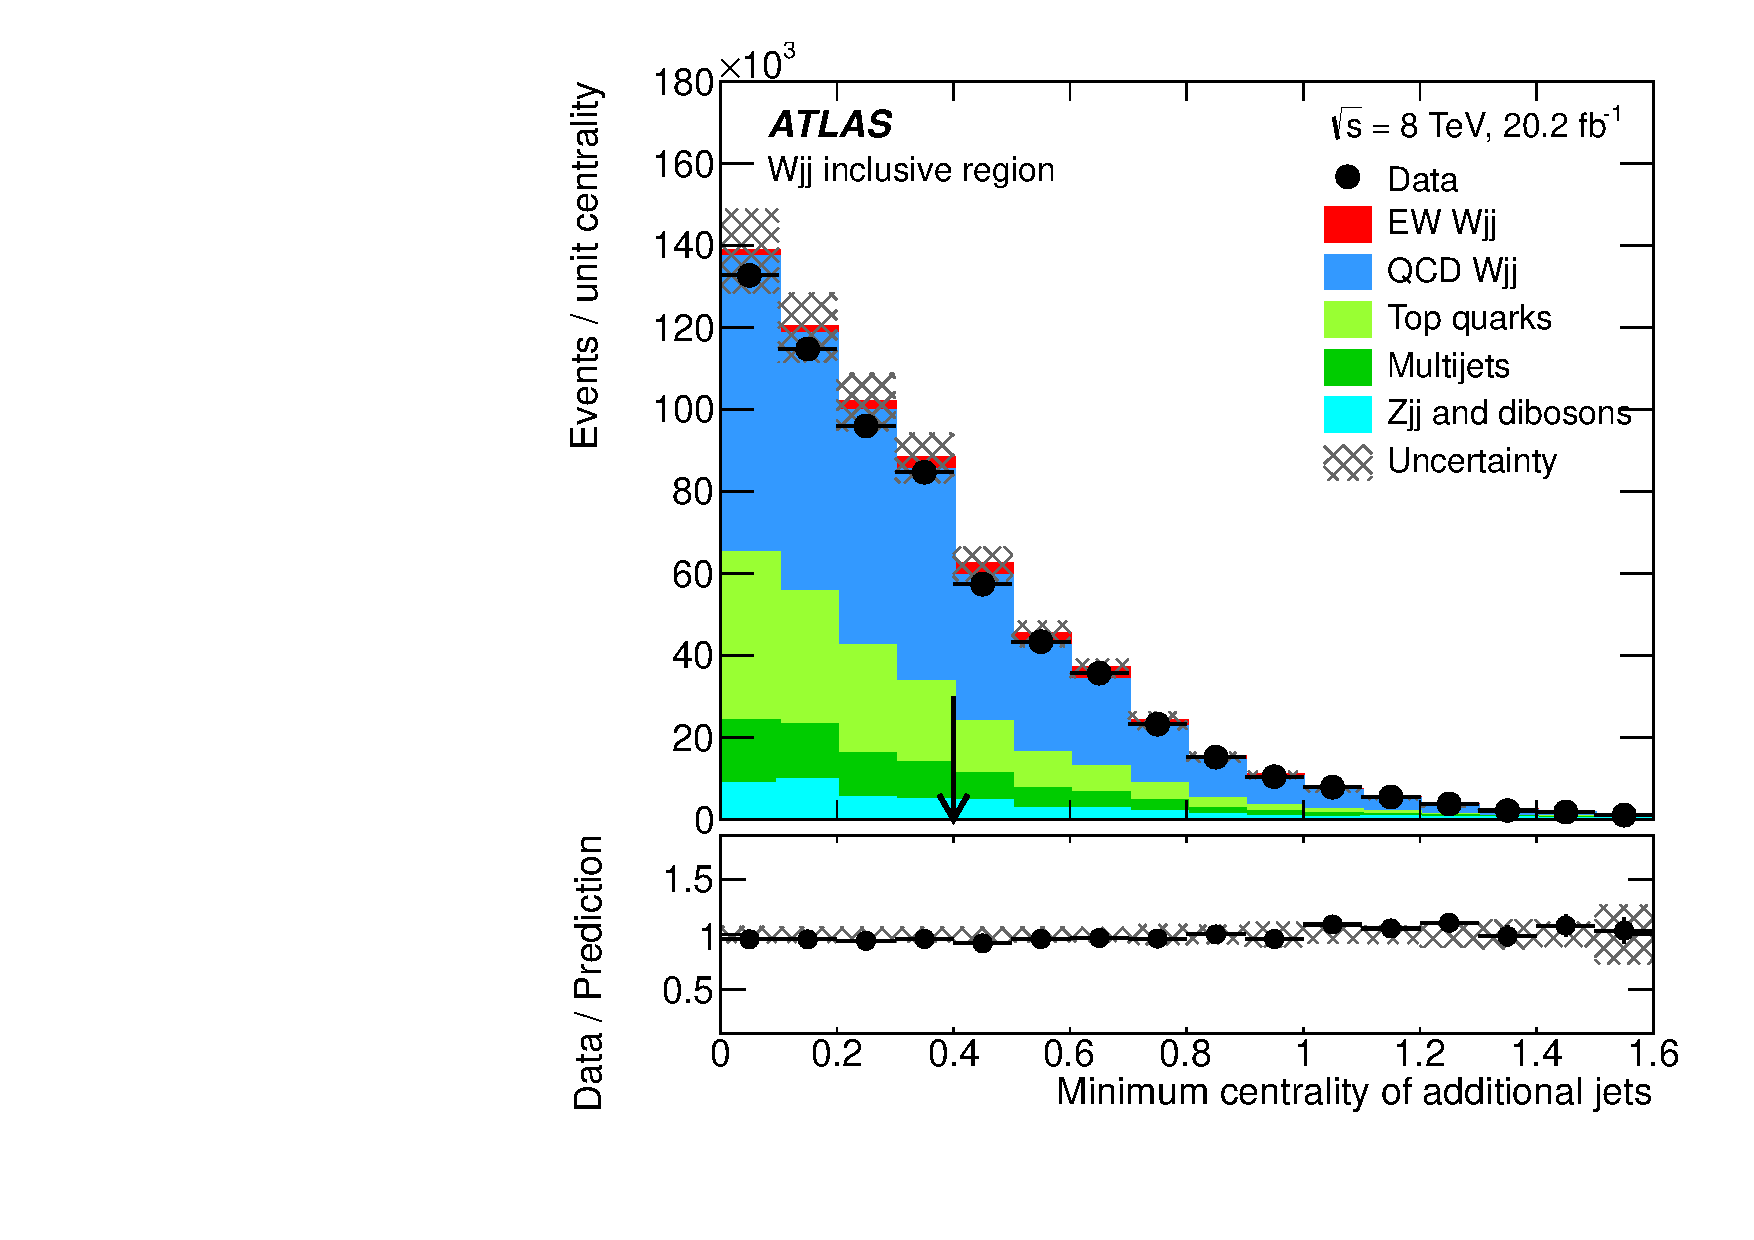
\includegraphics[width=.49\textwidth]{STDM-2014-11/fig_05d.pdf}
%%   \caption{Discriminating variables.}
%%   \label{wjj-discriminating-variables}
%% \end{figure}

Figure~\ref{wjj-mjj-distribution}.

\begin{figure}
\centering
  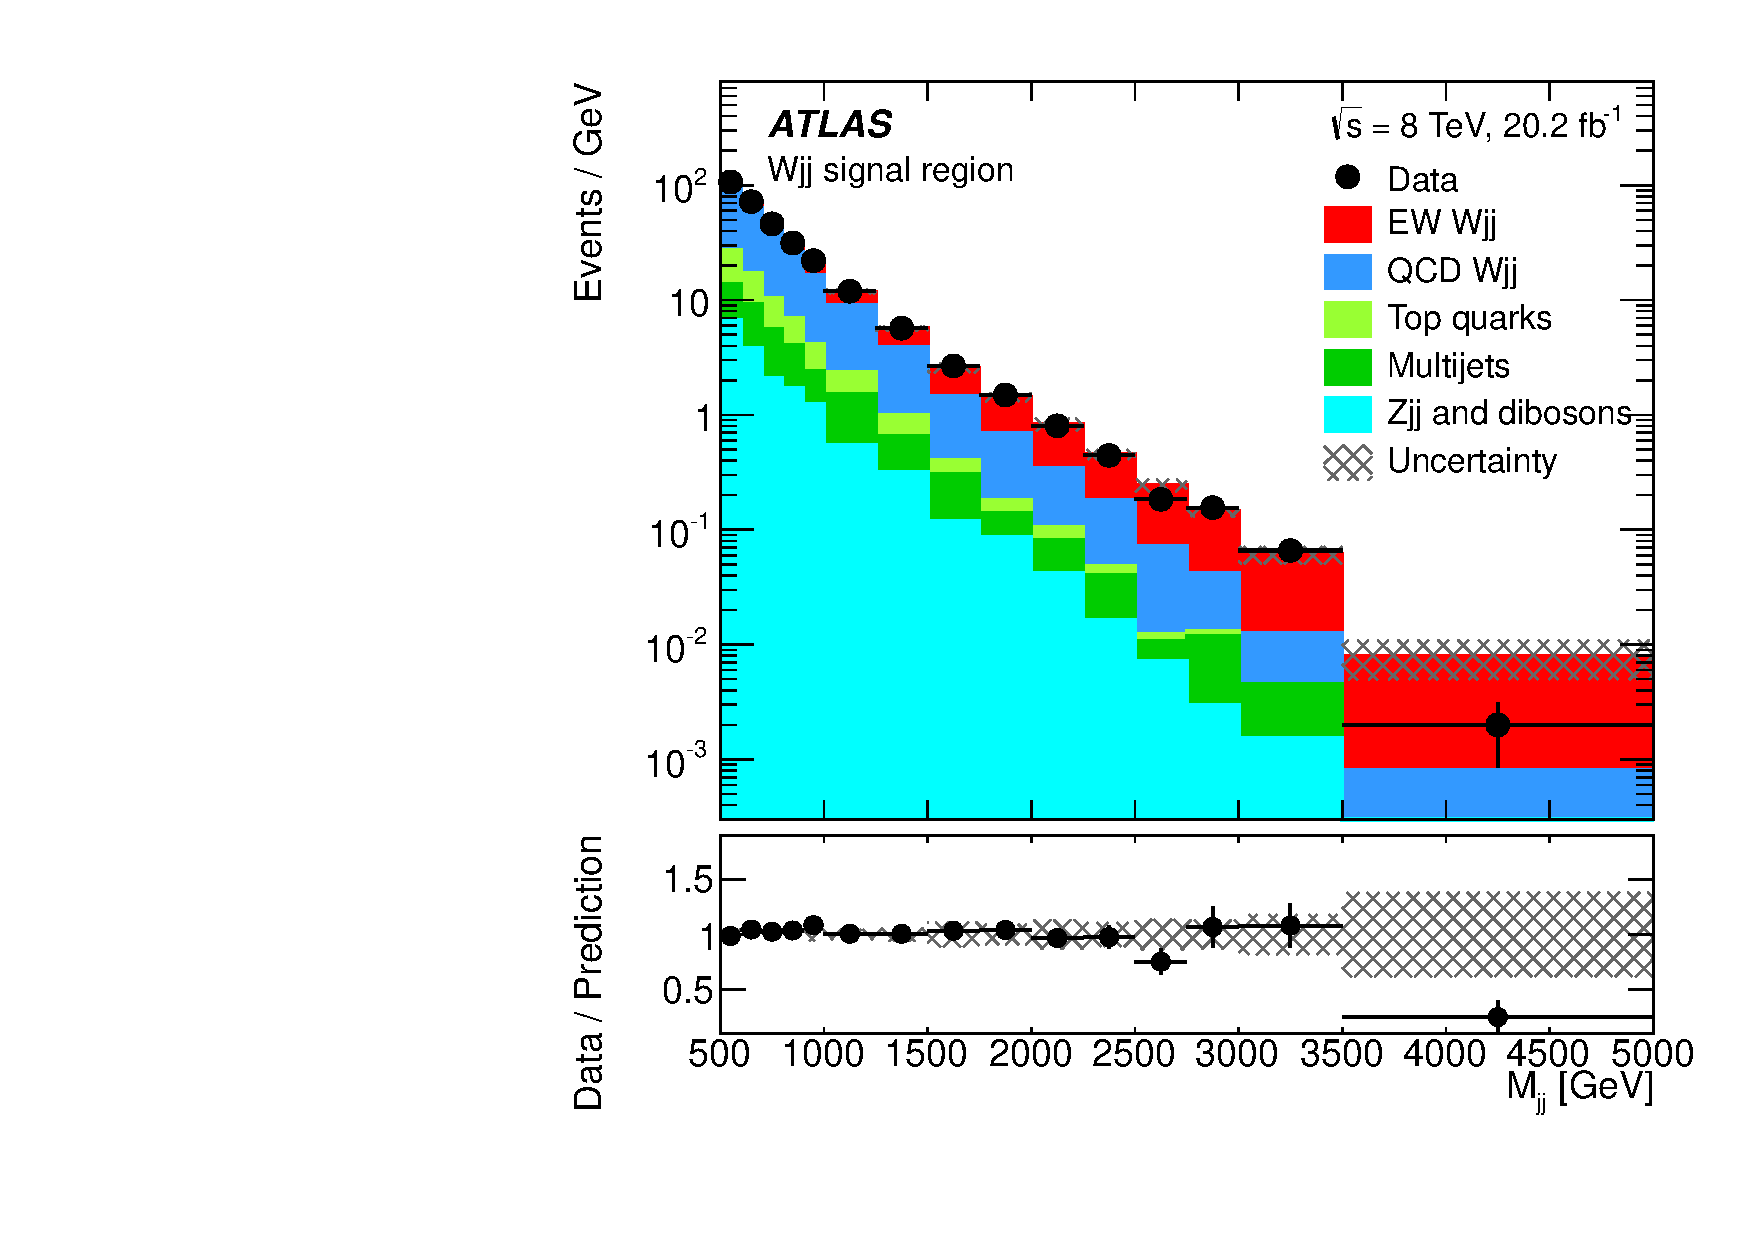
\includegraphics[width=.49\textwidth]{STDM-2014-11/fig_09b.pdf}
  \caption{The $m_{jj}$ distribution.}
  \label{wjj-mjj-distribution}
\end{figure}

Figure~\ref{wjj-differential-distributions}.

\begin{figure}
\centering
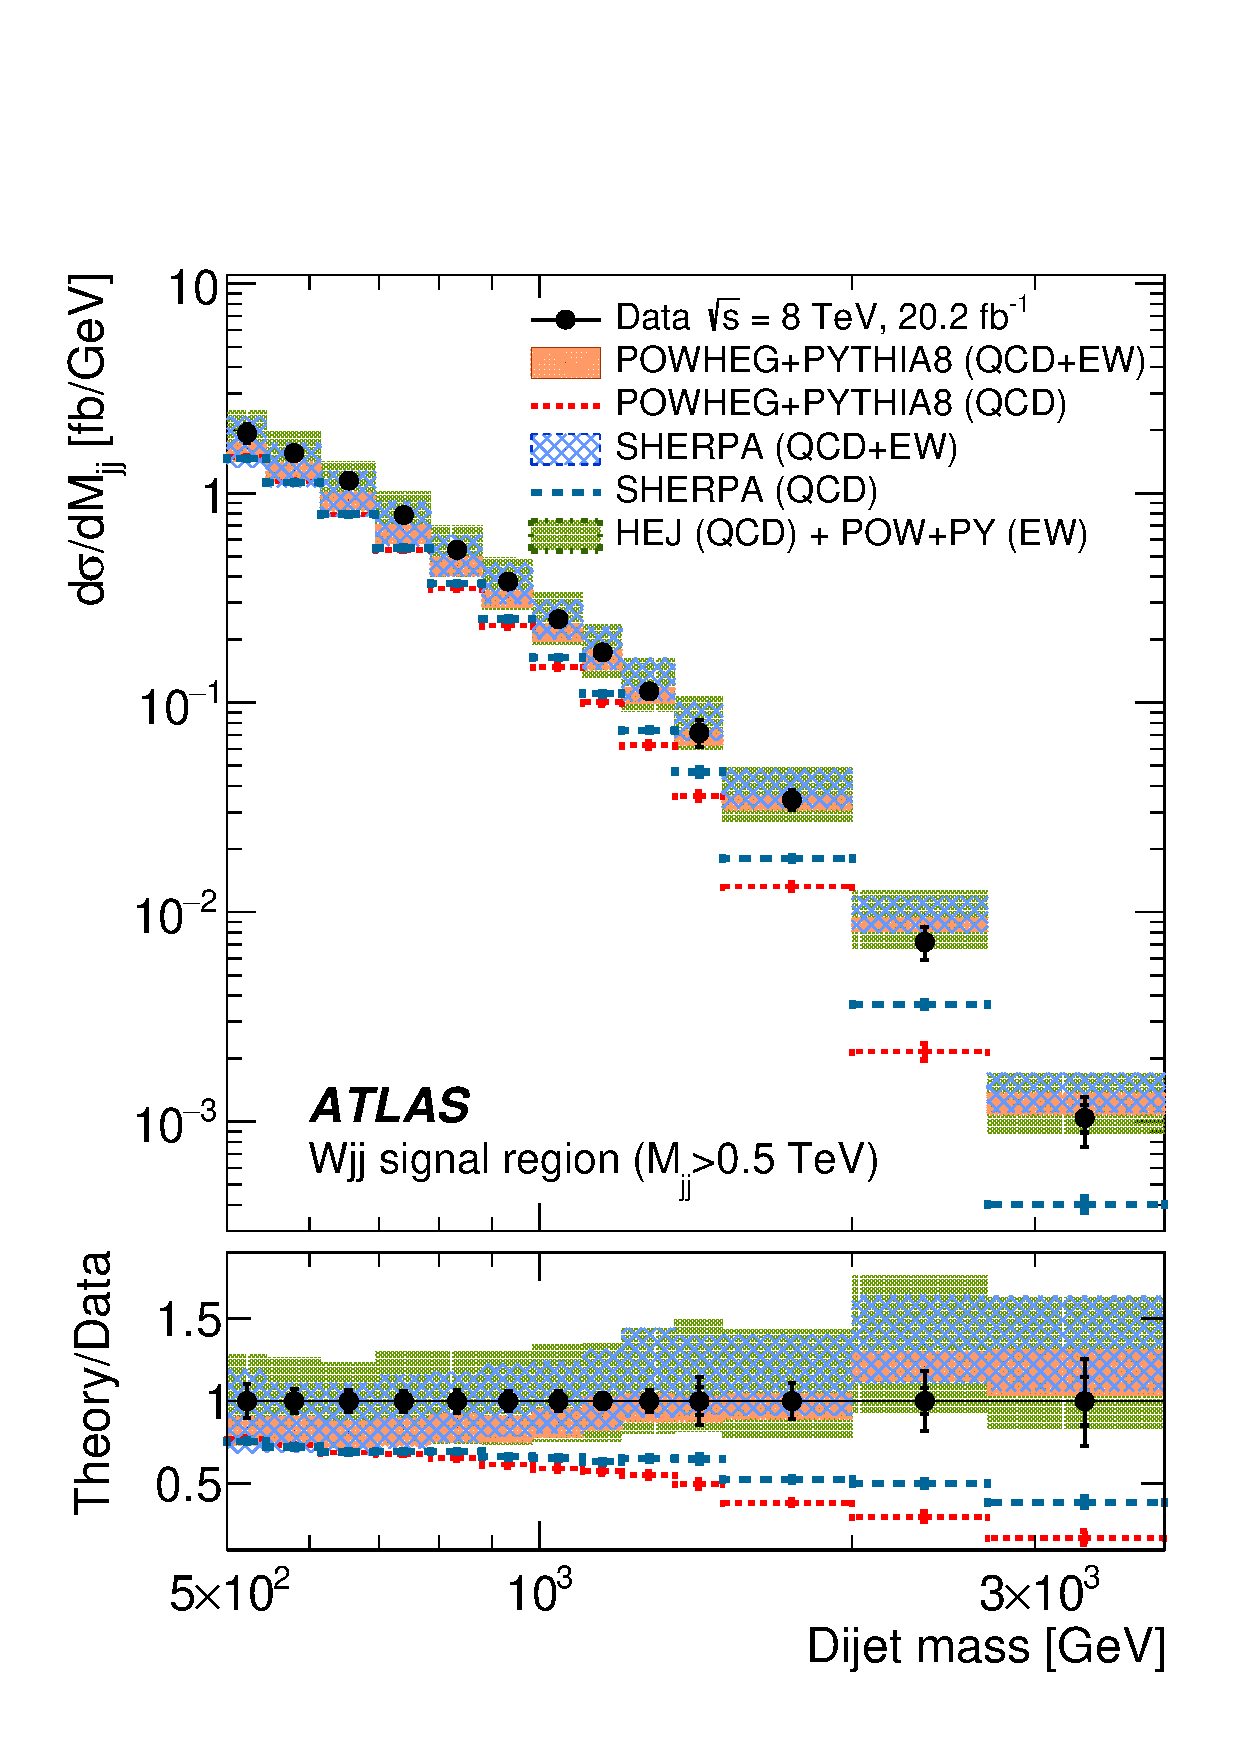
\includegraphics[width=.49\textwidth]{STDM-2014-11/fig_16a.pdf}
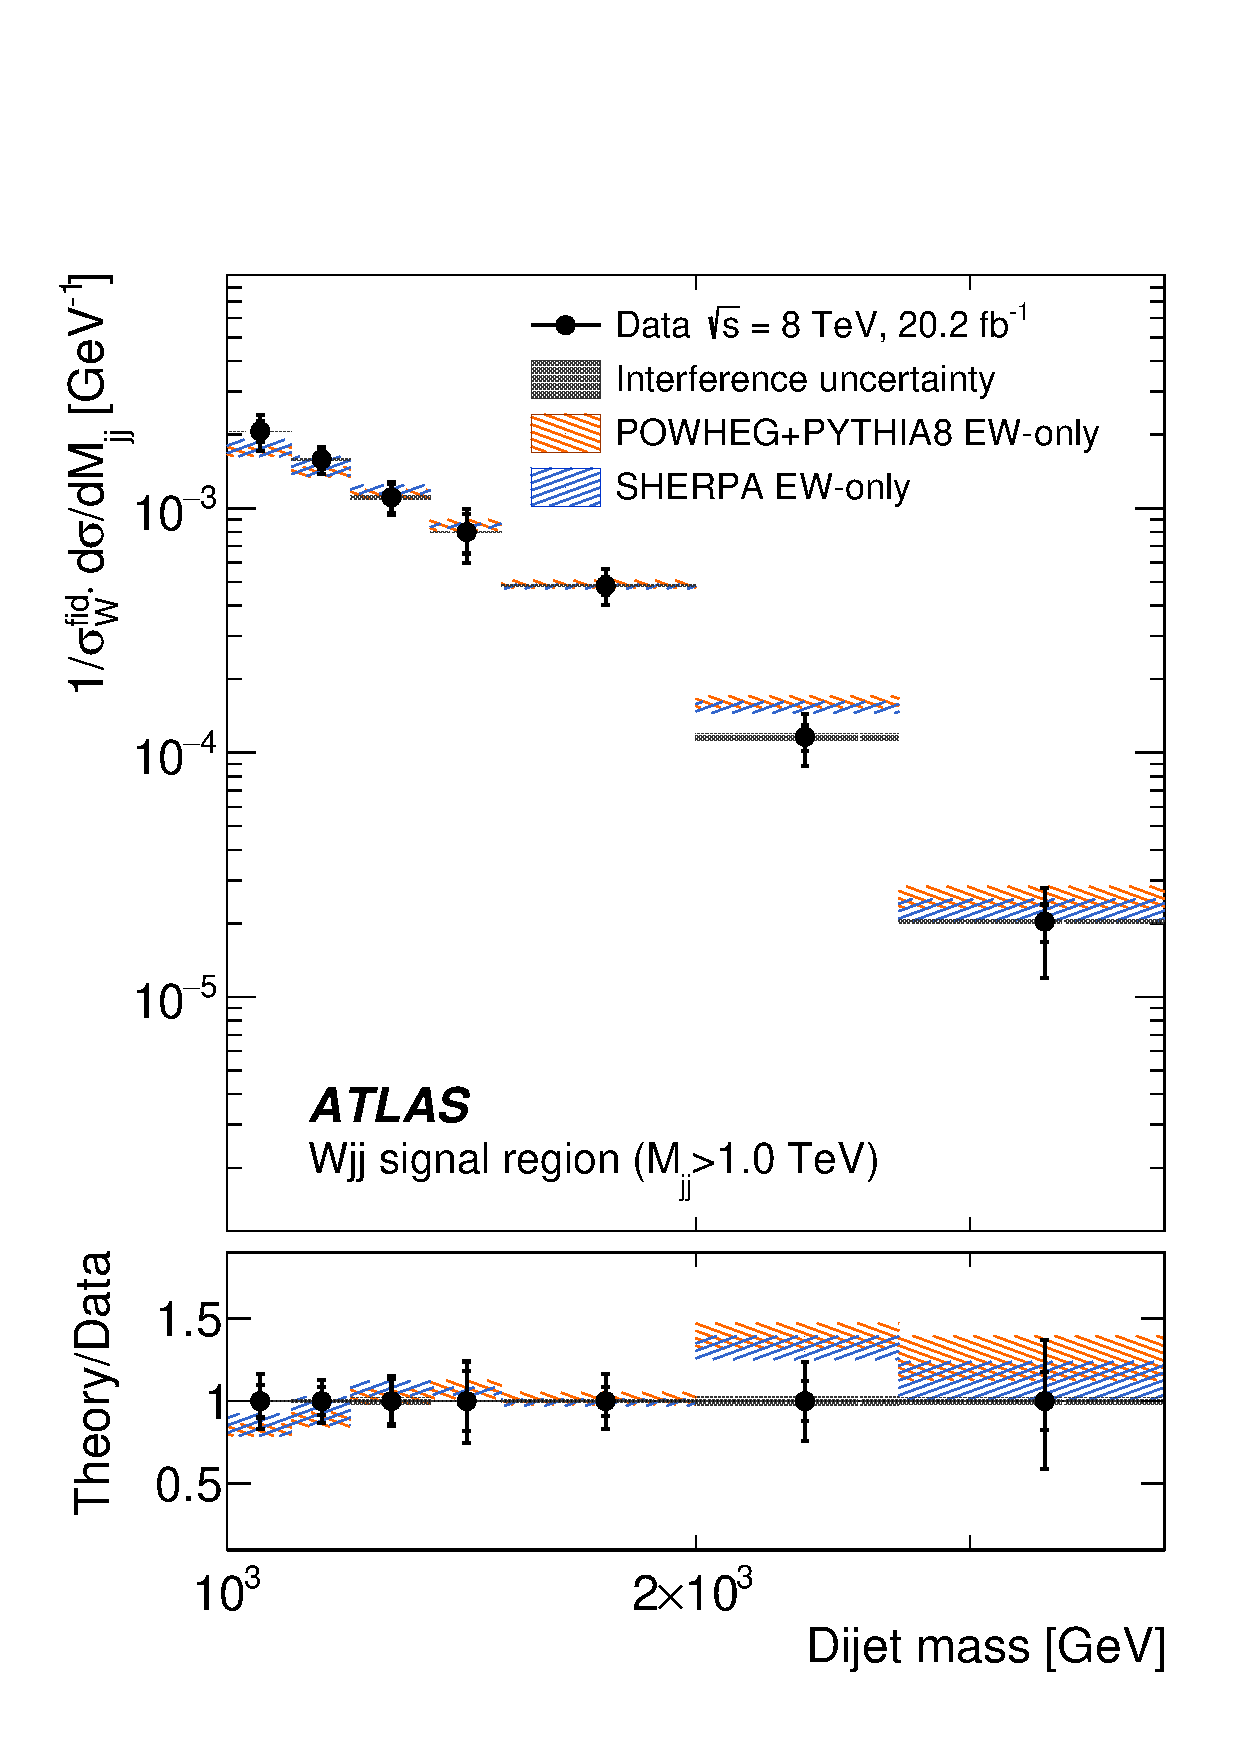
\includegraphics[width=.49\textwidth]{STDM-2014-11/fig_19b.pdf}
  \caption{\wjj differential distributions of the dijet mass in two fiducial regions. Left, the $\mjj$
    spectrum in the fiducial region $\mjj>0.5$~TeV. The QCD-only predictions (dashed lines) do not
    adequately describe the observed events; QCD+EW predictions agree well with the data.
    Right: the normalized differential distribution of the EW \wjj dijet spectrum in the region
    $\mjj>1.0$~TeV.
  }
  \label{wjj-differential-distributions}
\end{figure}

Figure~\ref{wjj-atgc}.

%% \begin{figure}
%% 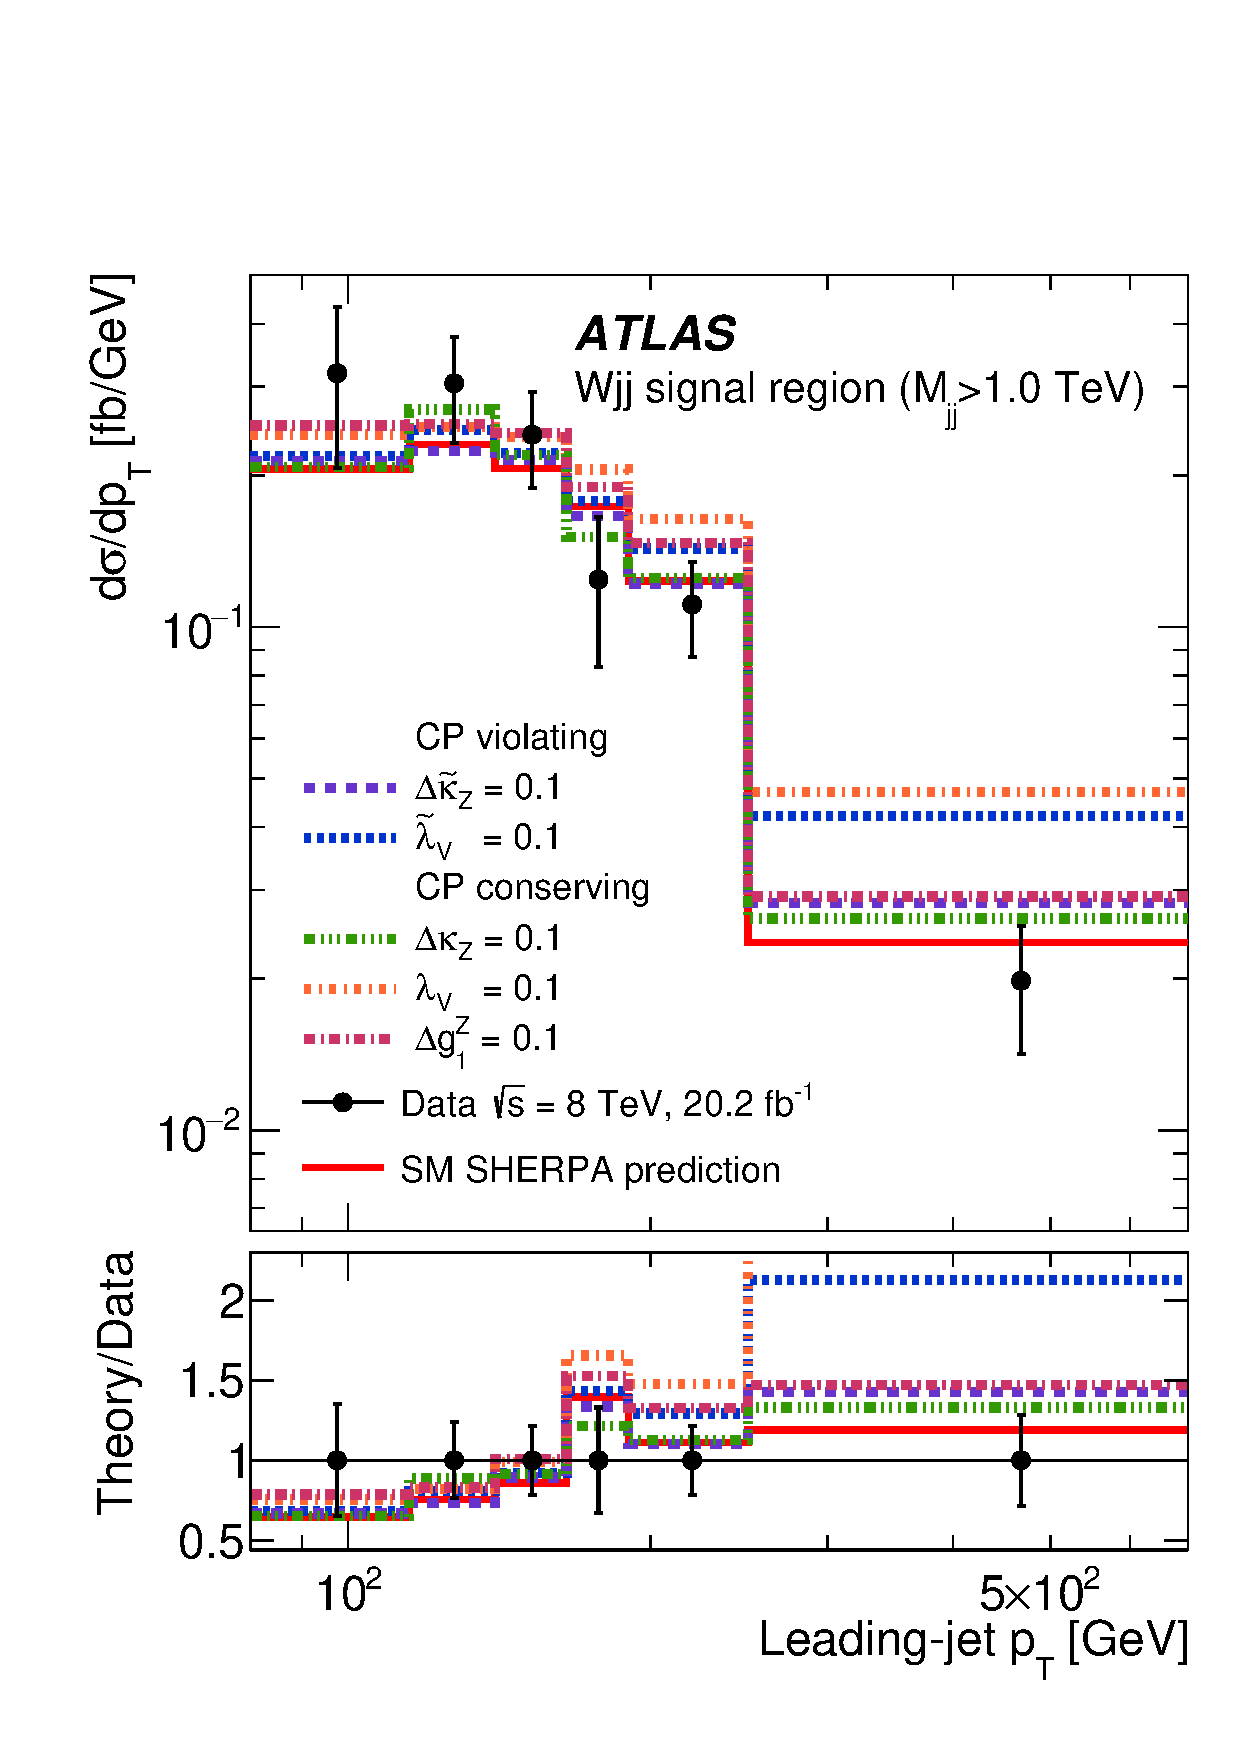
\includegraphics[width=.49\textwidth]{STDM-2014-11/figaux_30b.pdf}
%%   \caption{Anomalous triple gauge couplings.}
%%   \label{wjj-atgc}
%% \end{figure}

%% \begin{figure}
%% 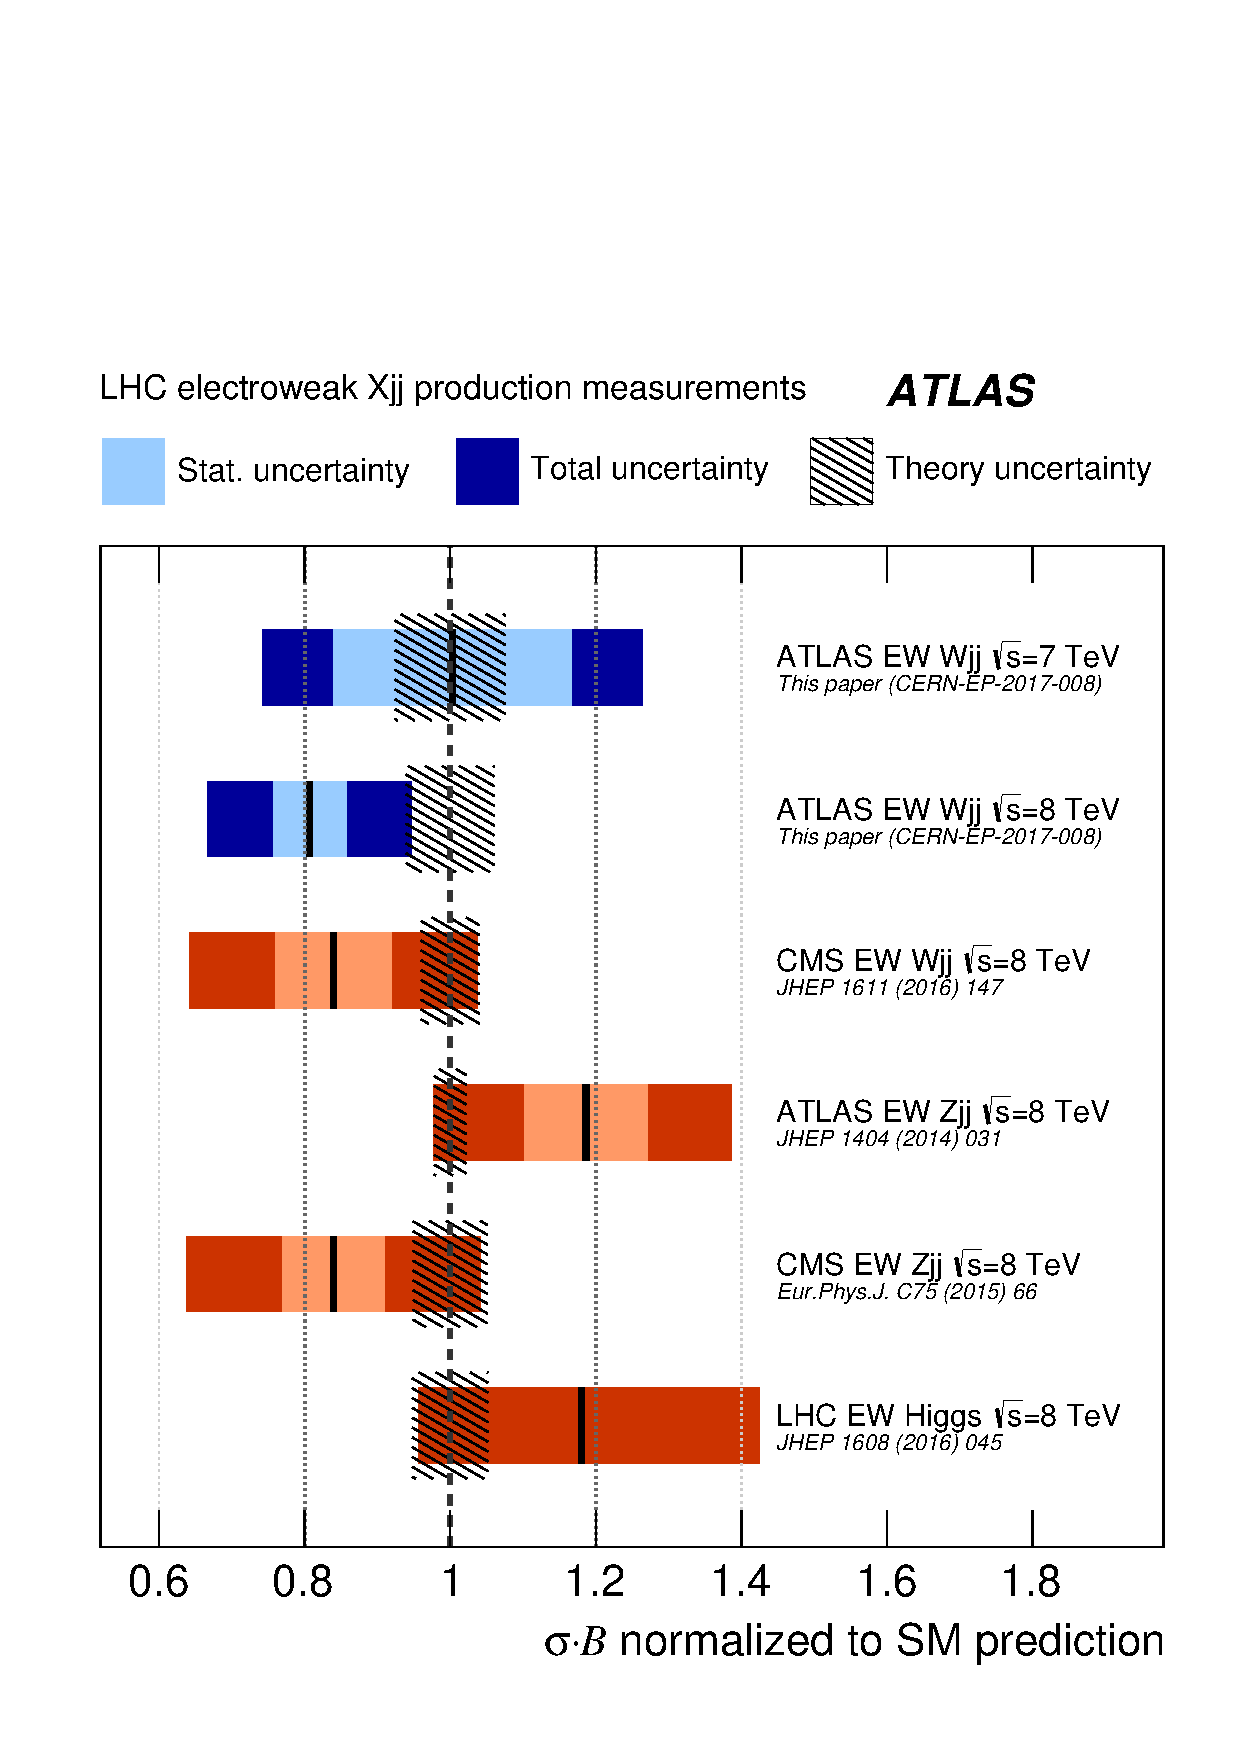
\includegraphics[width=.49\textwidth]{STDM-2014-11/fig_10.pdf}
%%   \caption{LHC electroweak Xjj production measurments (according to the 8 TeV paper).}
%%   \label{wjj-summary}
%% \end{figure}



\section{\zjj Production Measurement}

Figure~\ref{zjj-dijet-mismodeling} describes blah.

%% \begin{figure}
%% \centering
%%   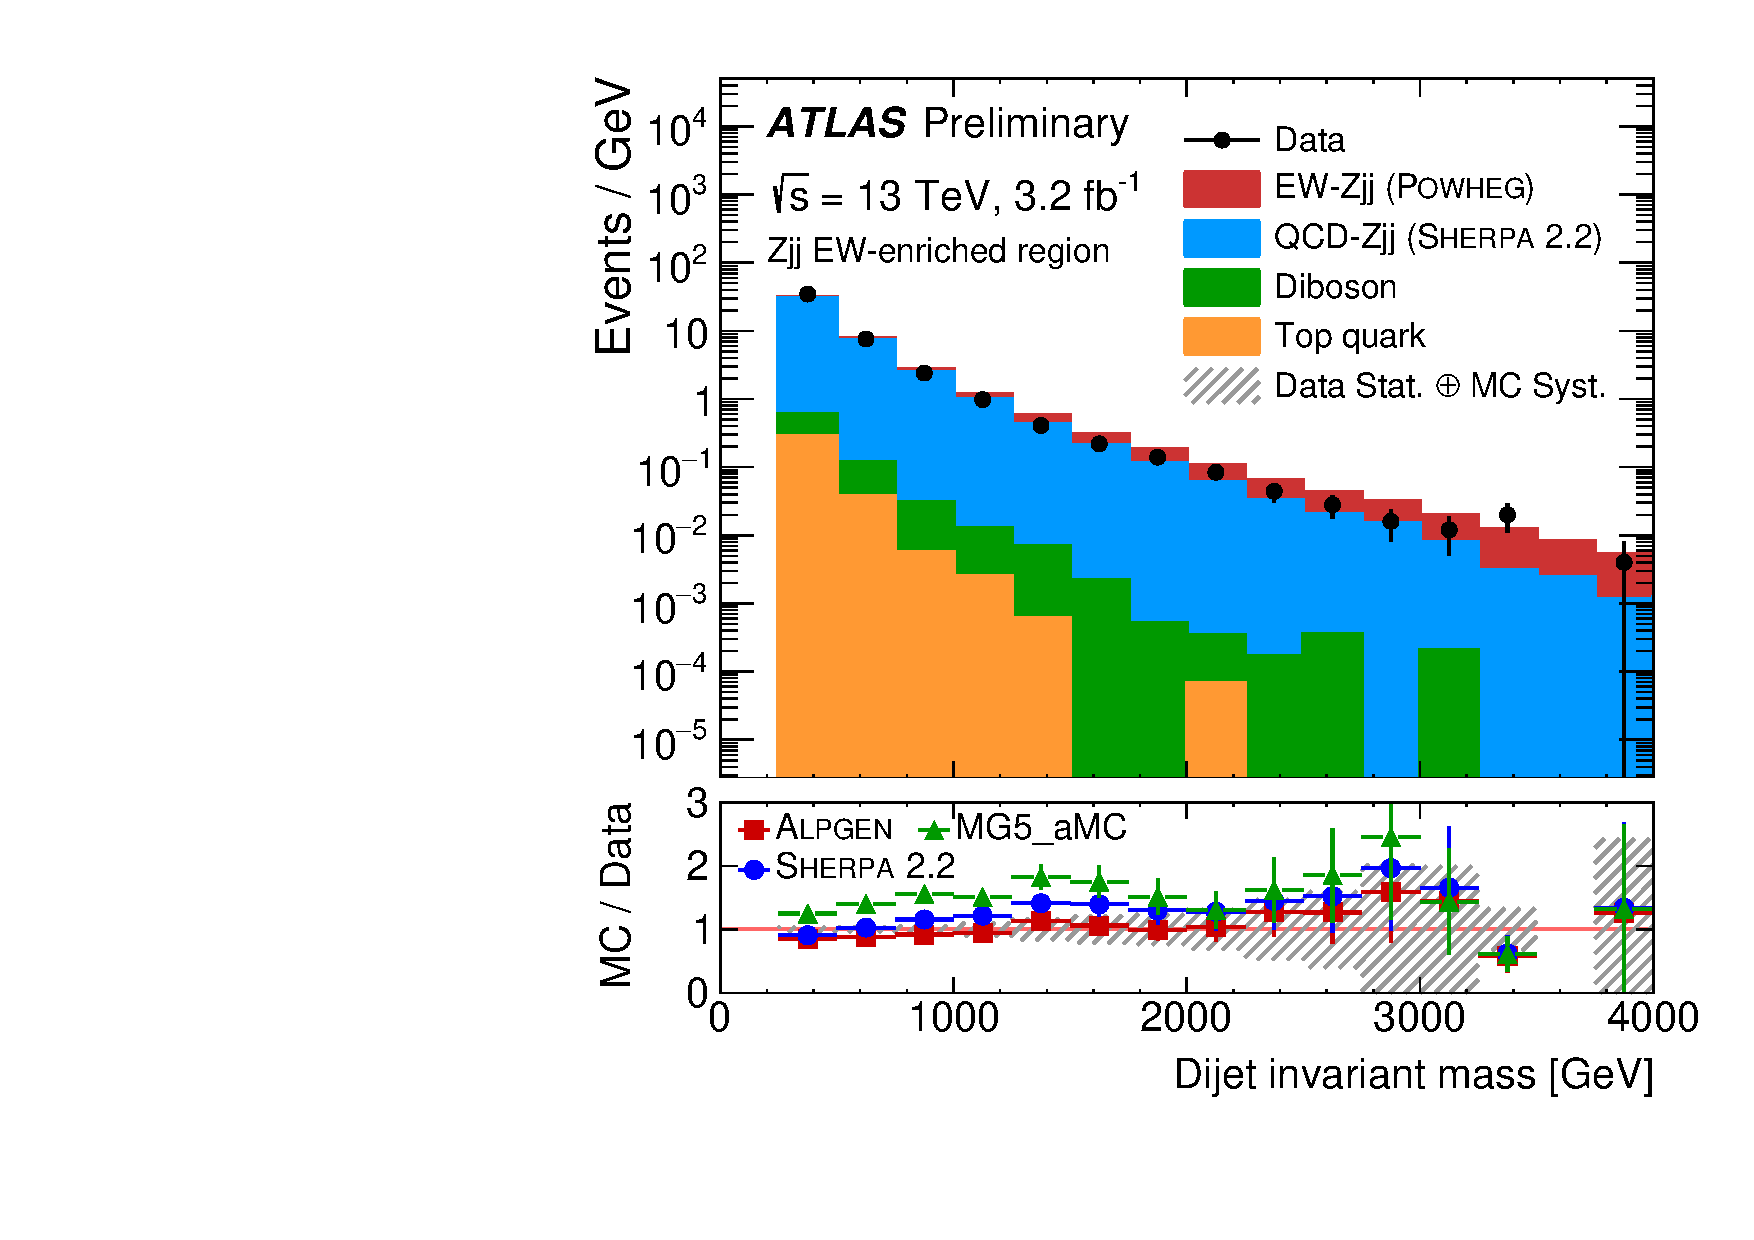
\includegraphics[width=.33\textwidth]{STDM-2016-09/fig_02a.pdf}
%%   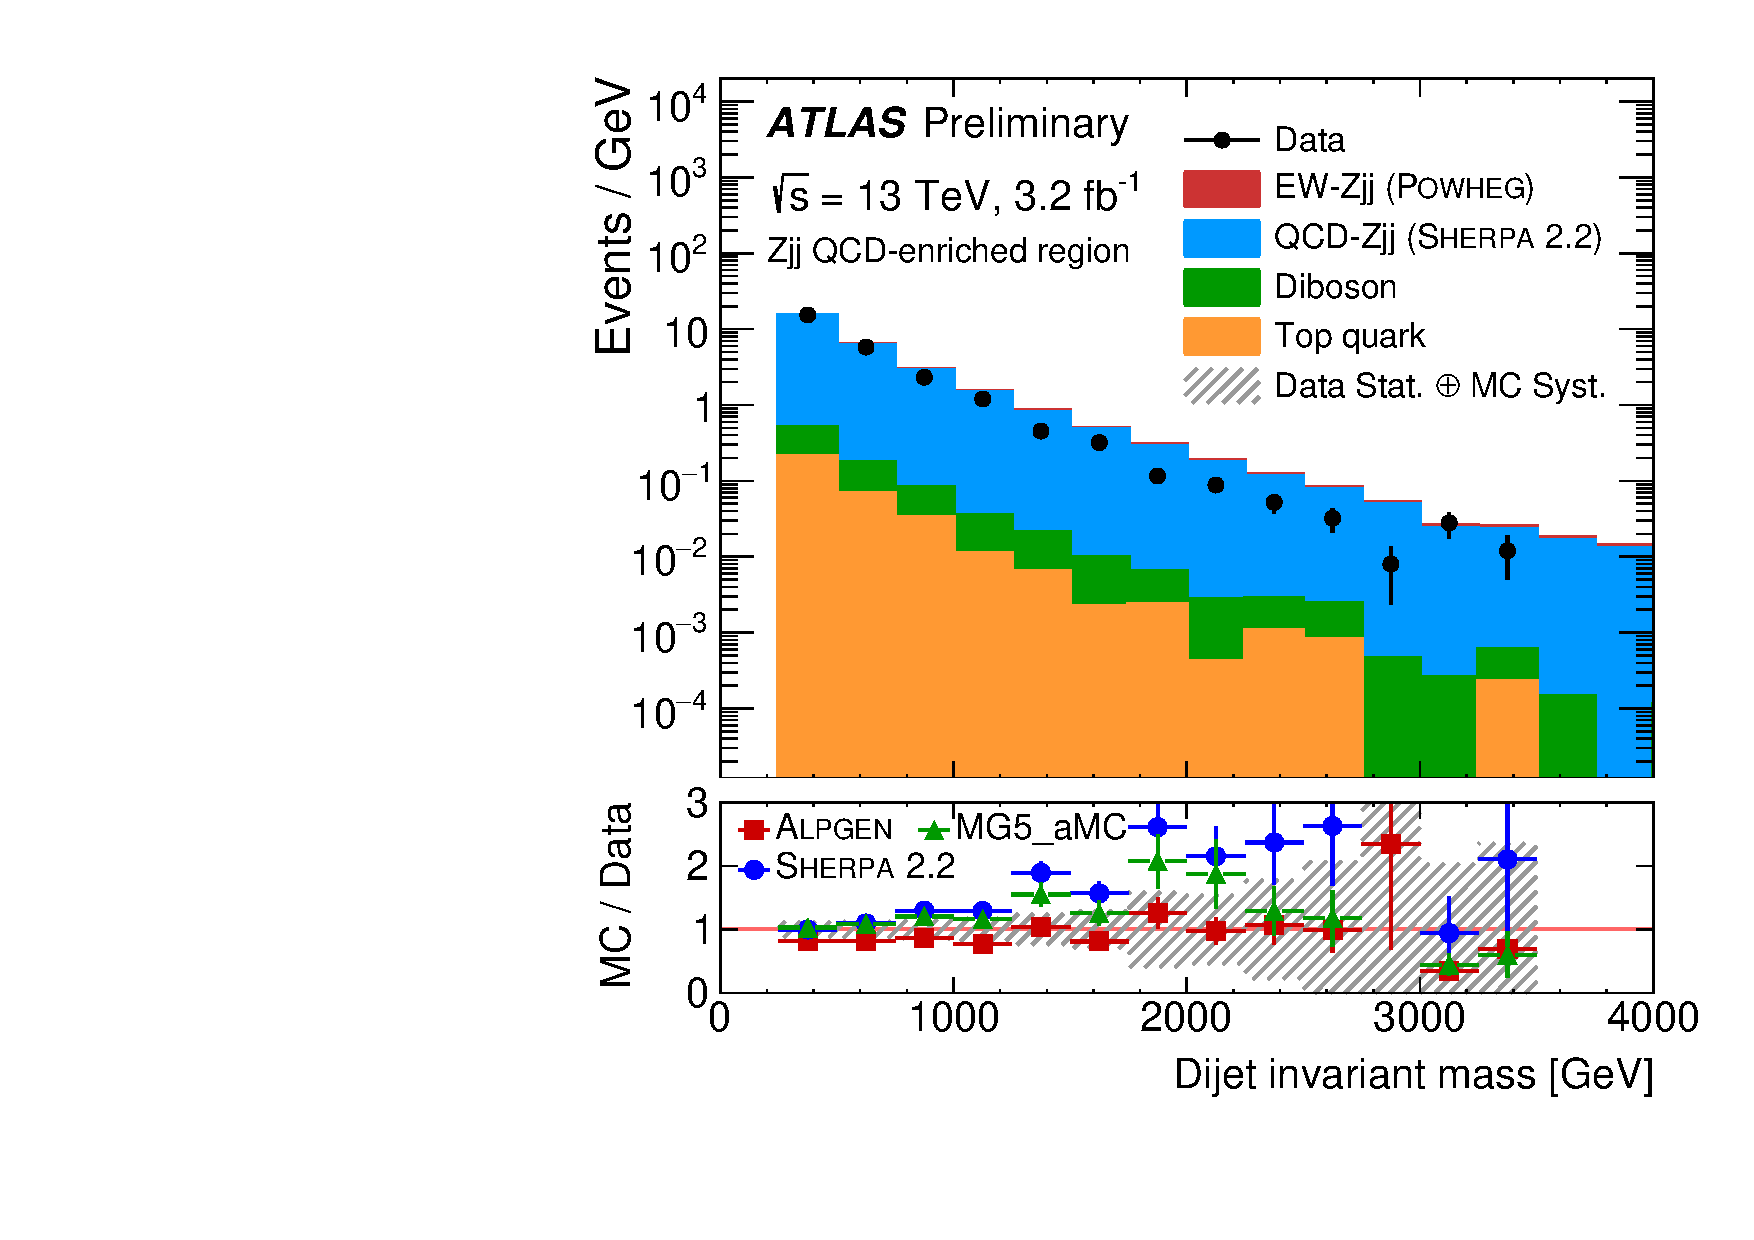
\includegraphics[width=.33\textwidth]{STDM-2016-09/fig_02b.pdf}
%%   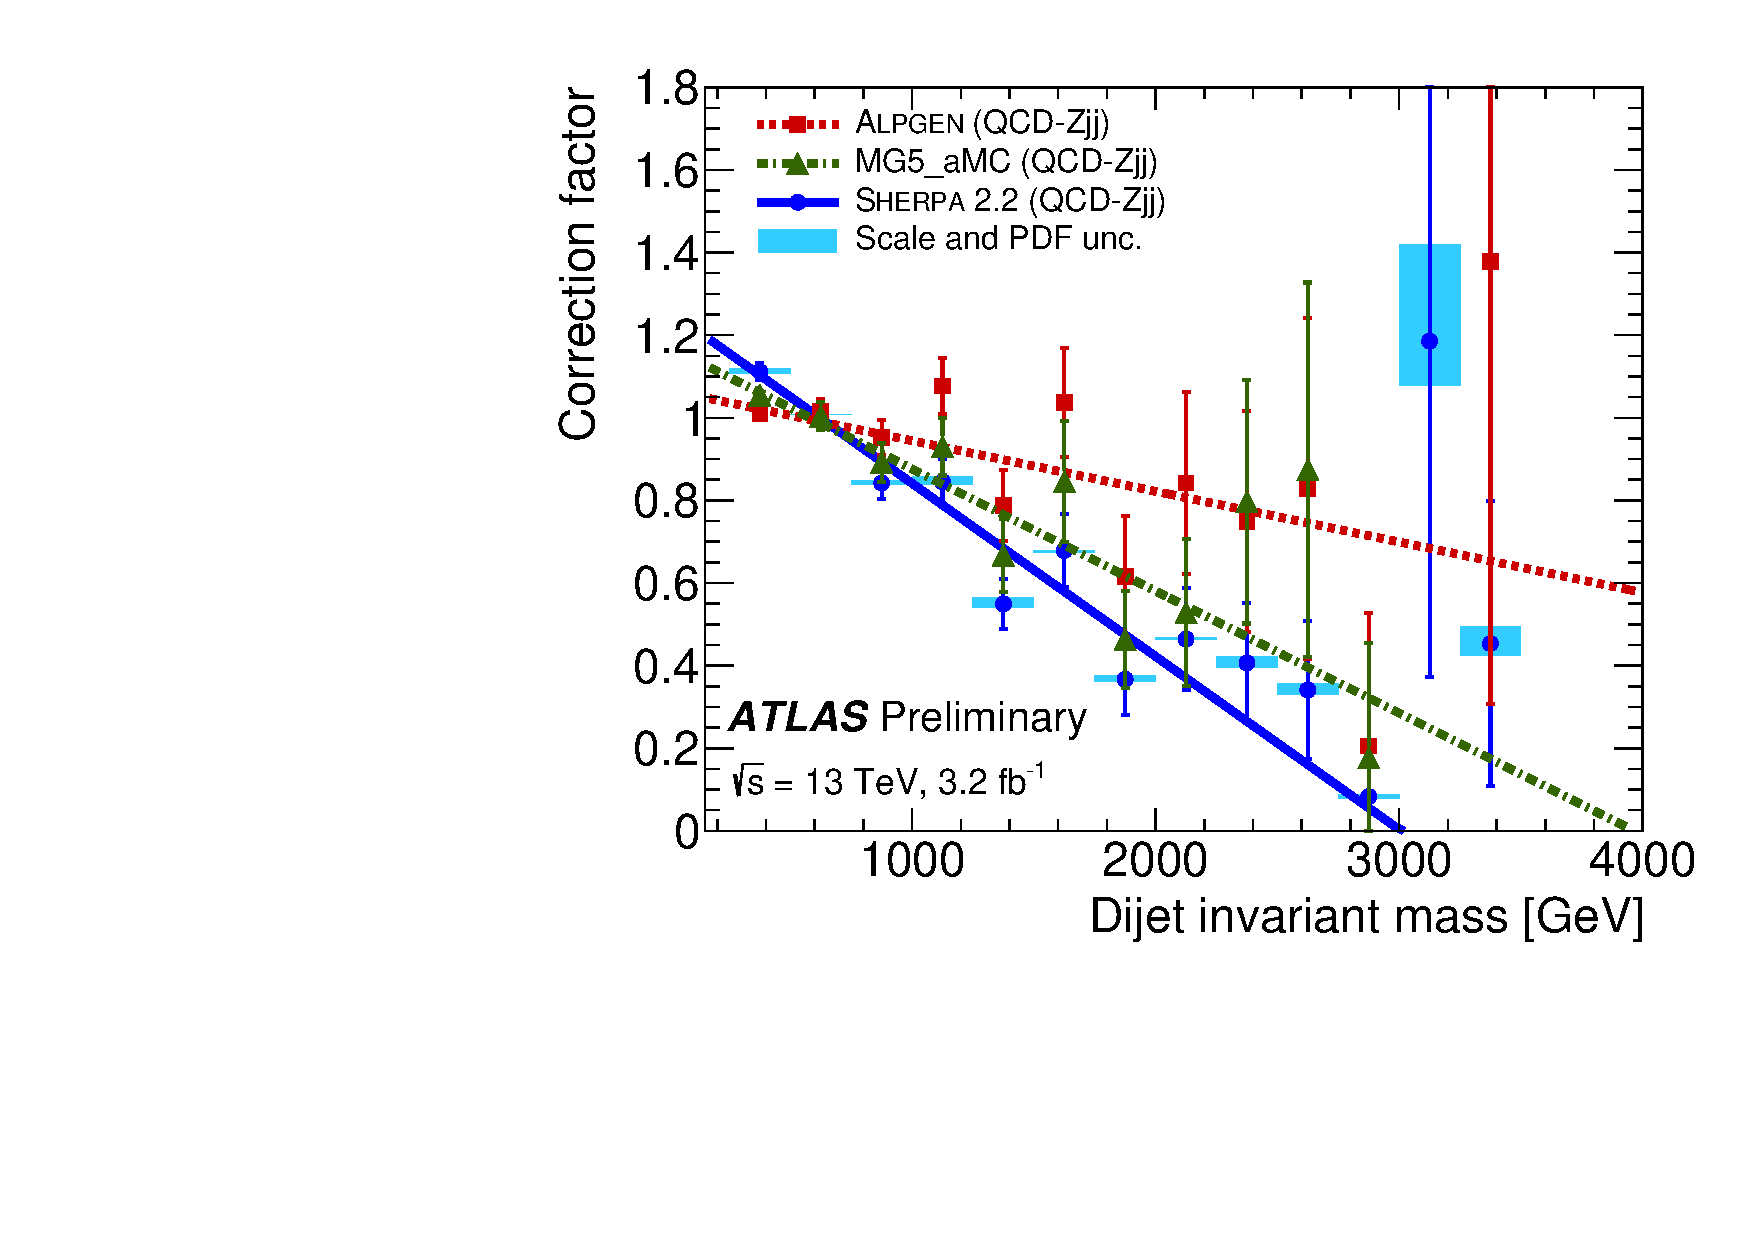
\includegraphics[width=.33\textwidth]{STDM-2016-09/fig_03a.pdf}
%%   \caption{$M_{jj}$ distribution.}
%%   \label{zjj-dijet-mismodeling}
%% \end{figure}

Figure~\ref{zjj-dijet-post-fit}.

\begin{figure}
  \centering
  \begin{subfigure}[t]{0.50\textwidth}
  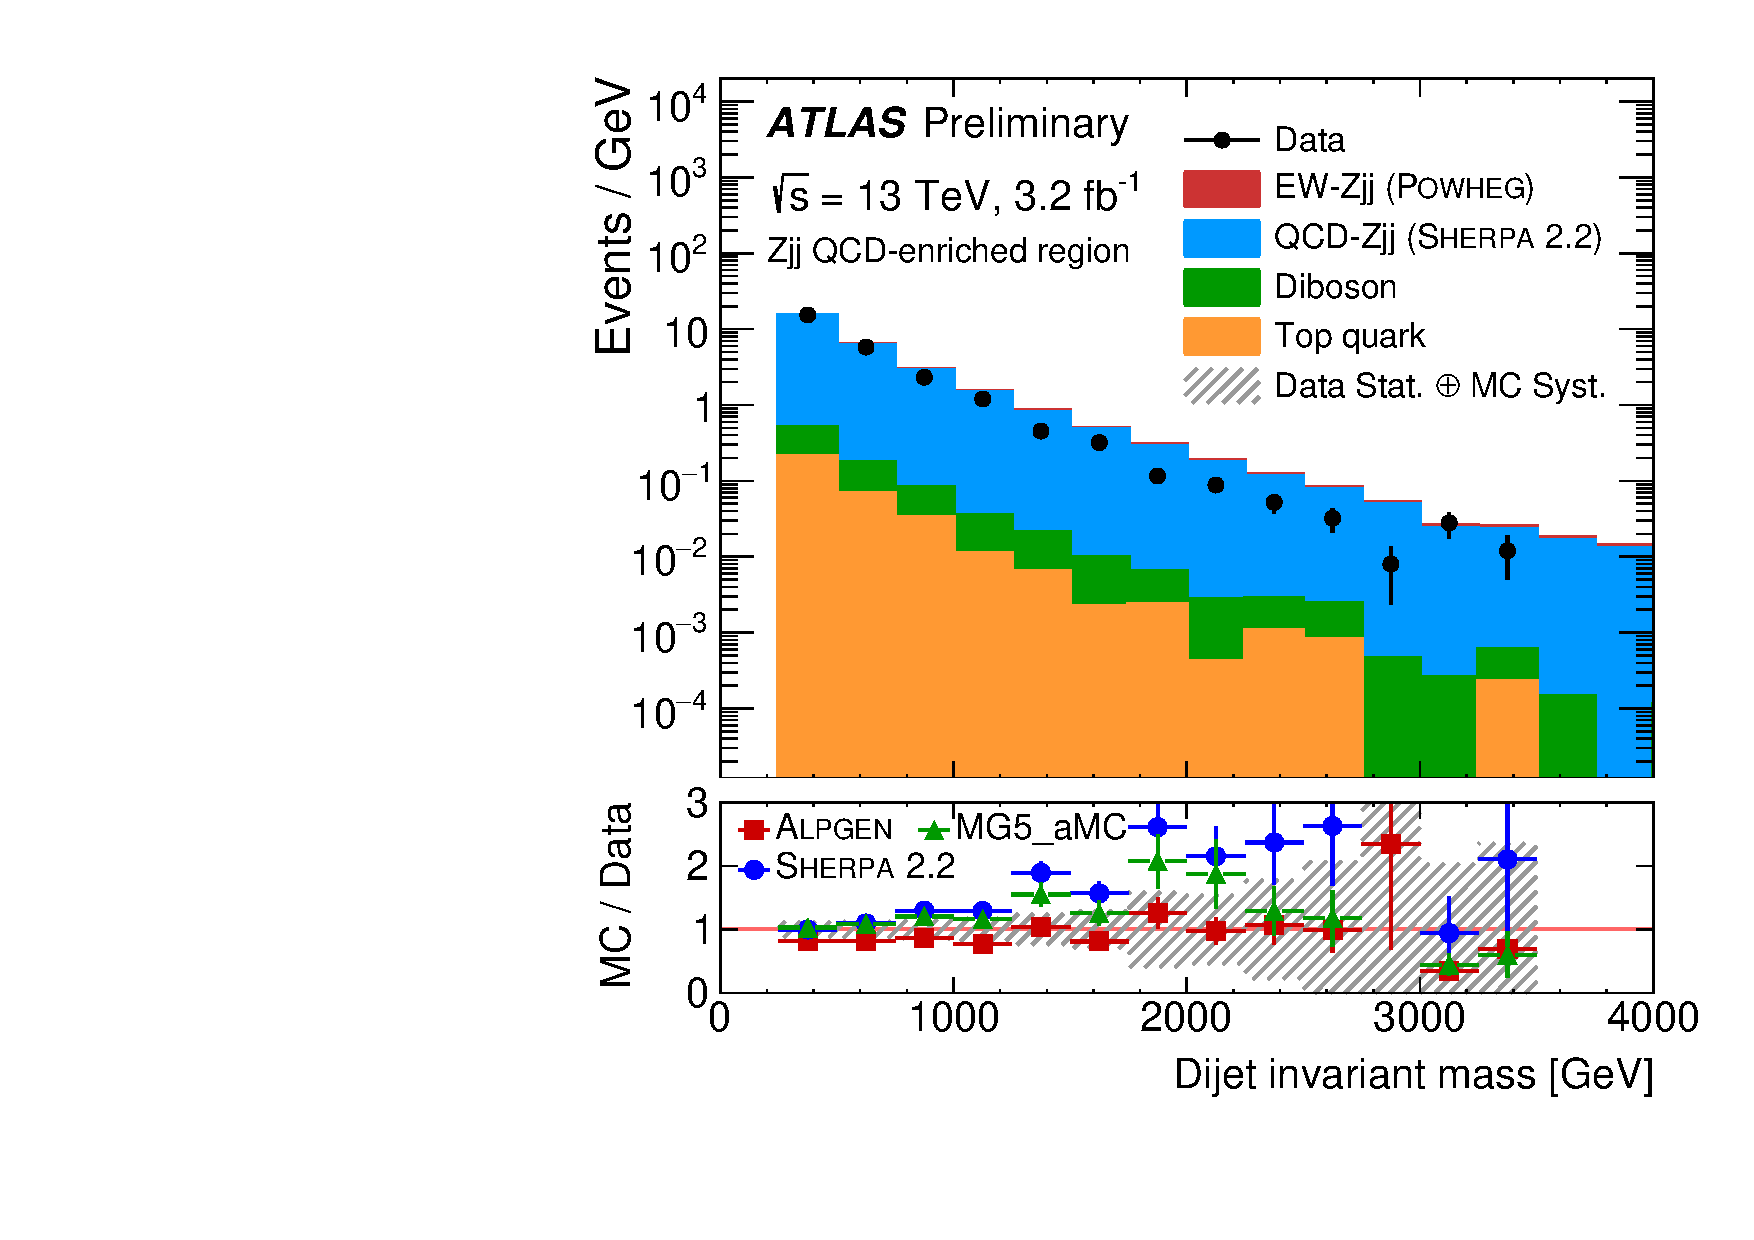
\includegraphics[width=.99\textwidth]{STDM-2016-09/fig_02b.pdf}\vspace{-6mm}
  \caption{}
  \end{subfigure}%
  ~
  \begin{subfigure}[t]{0.50\textwidth}
    \raisebox{0.15\height}{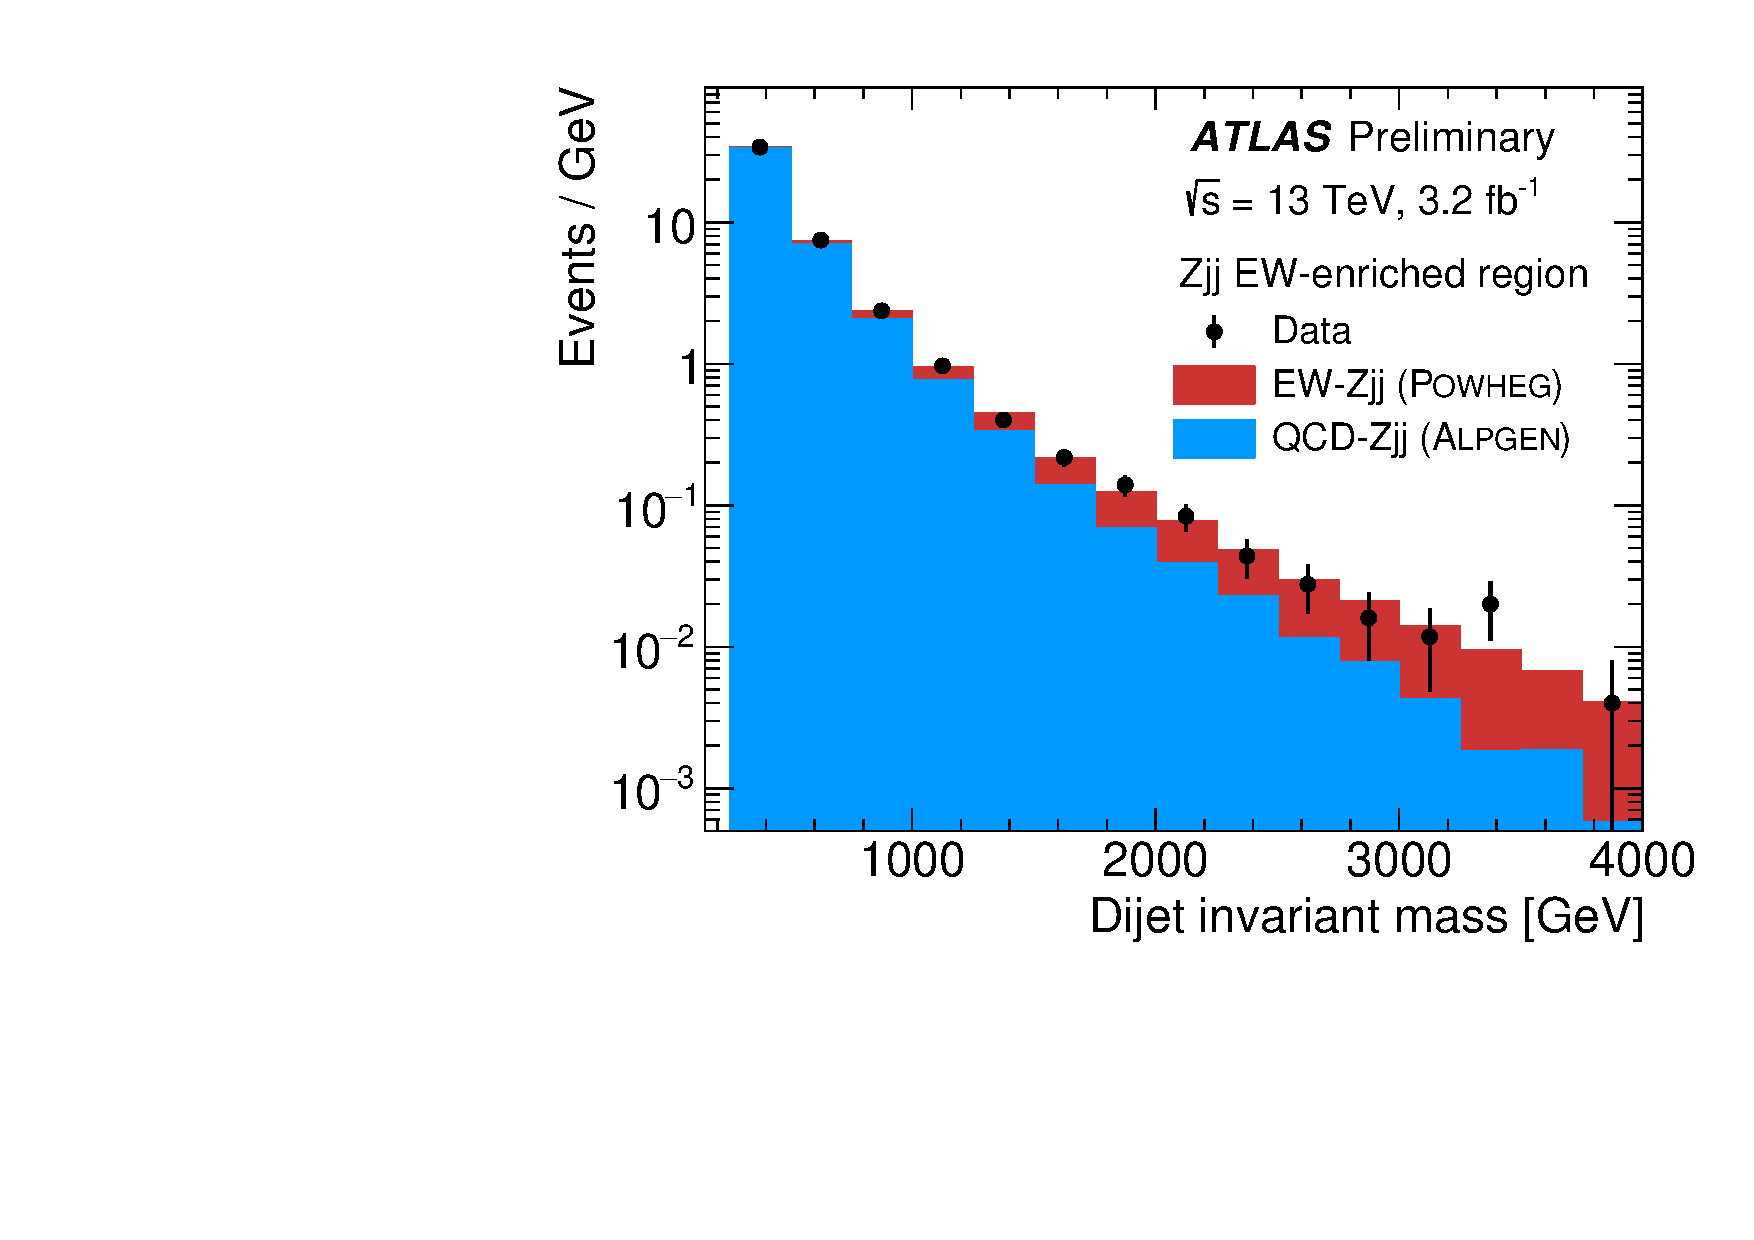
\includegraphics[width=.99\textwidth]{STDM-2016-09/fig_04a.pdf}}\vspace{-6mm}
%%   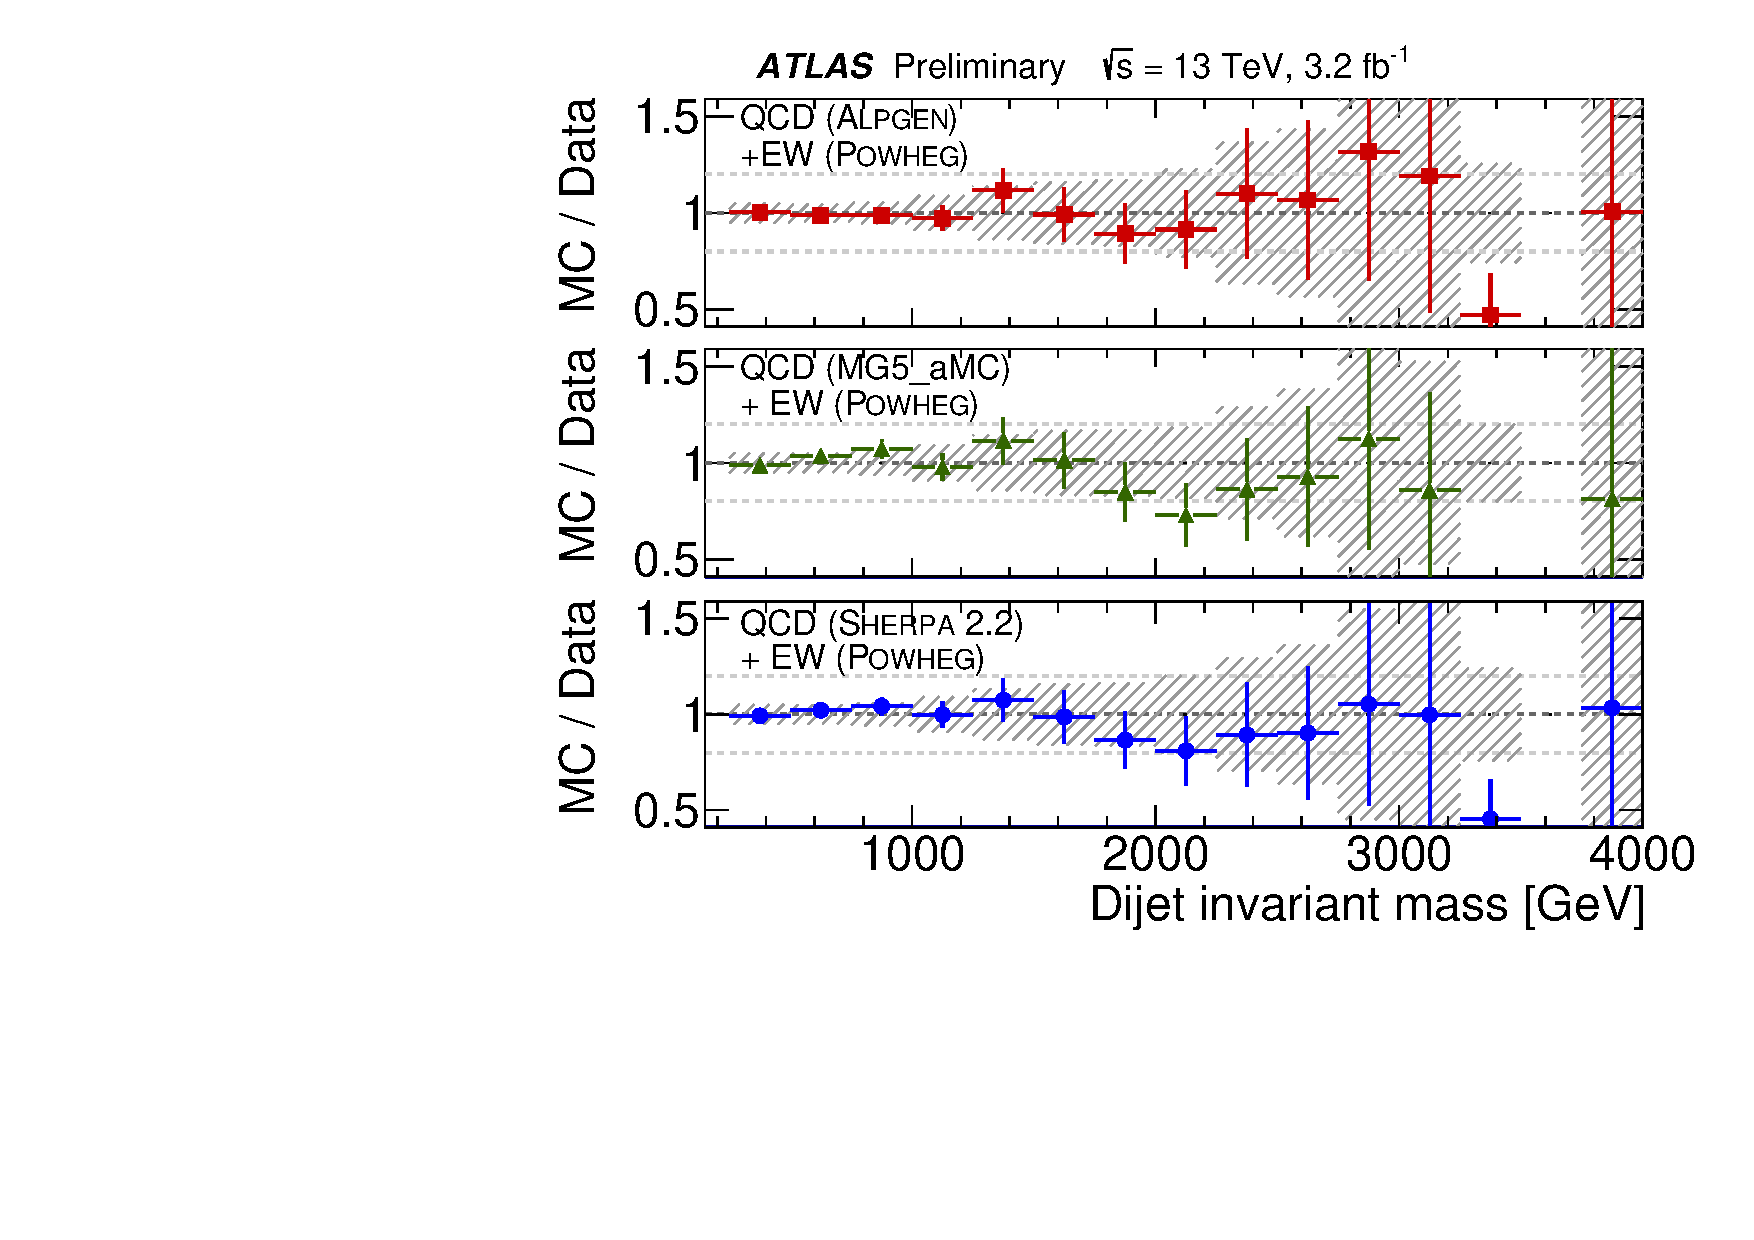
\includegraphics[width=.49\textwidth]{STDM-2016-09/fig_04b.pdf}
  \caption{}
  \end{subfigure}%
  \caption{(a) The dijet invariant mass \mjj in the \zjj QCD-enriched control region, which illustrates
the mismodeling of this observable by three MC generators. This region is used to derive a data-MC
correction factor that is applied to the QCD MC shape in the signal region.
(b) The QCD and EW templates from MC are fit to the data (minus non-\zjj background) to obtain the
cross section of each component.
}
  \label{zjj-dijet-post-fit}
\end{figure}

\section{Summary}

These results are consistent with Standard Model expectations.

Figure~\ref{zjj-wjj-summary-results}

\begin{figure}
\centering
  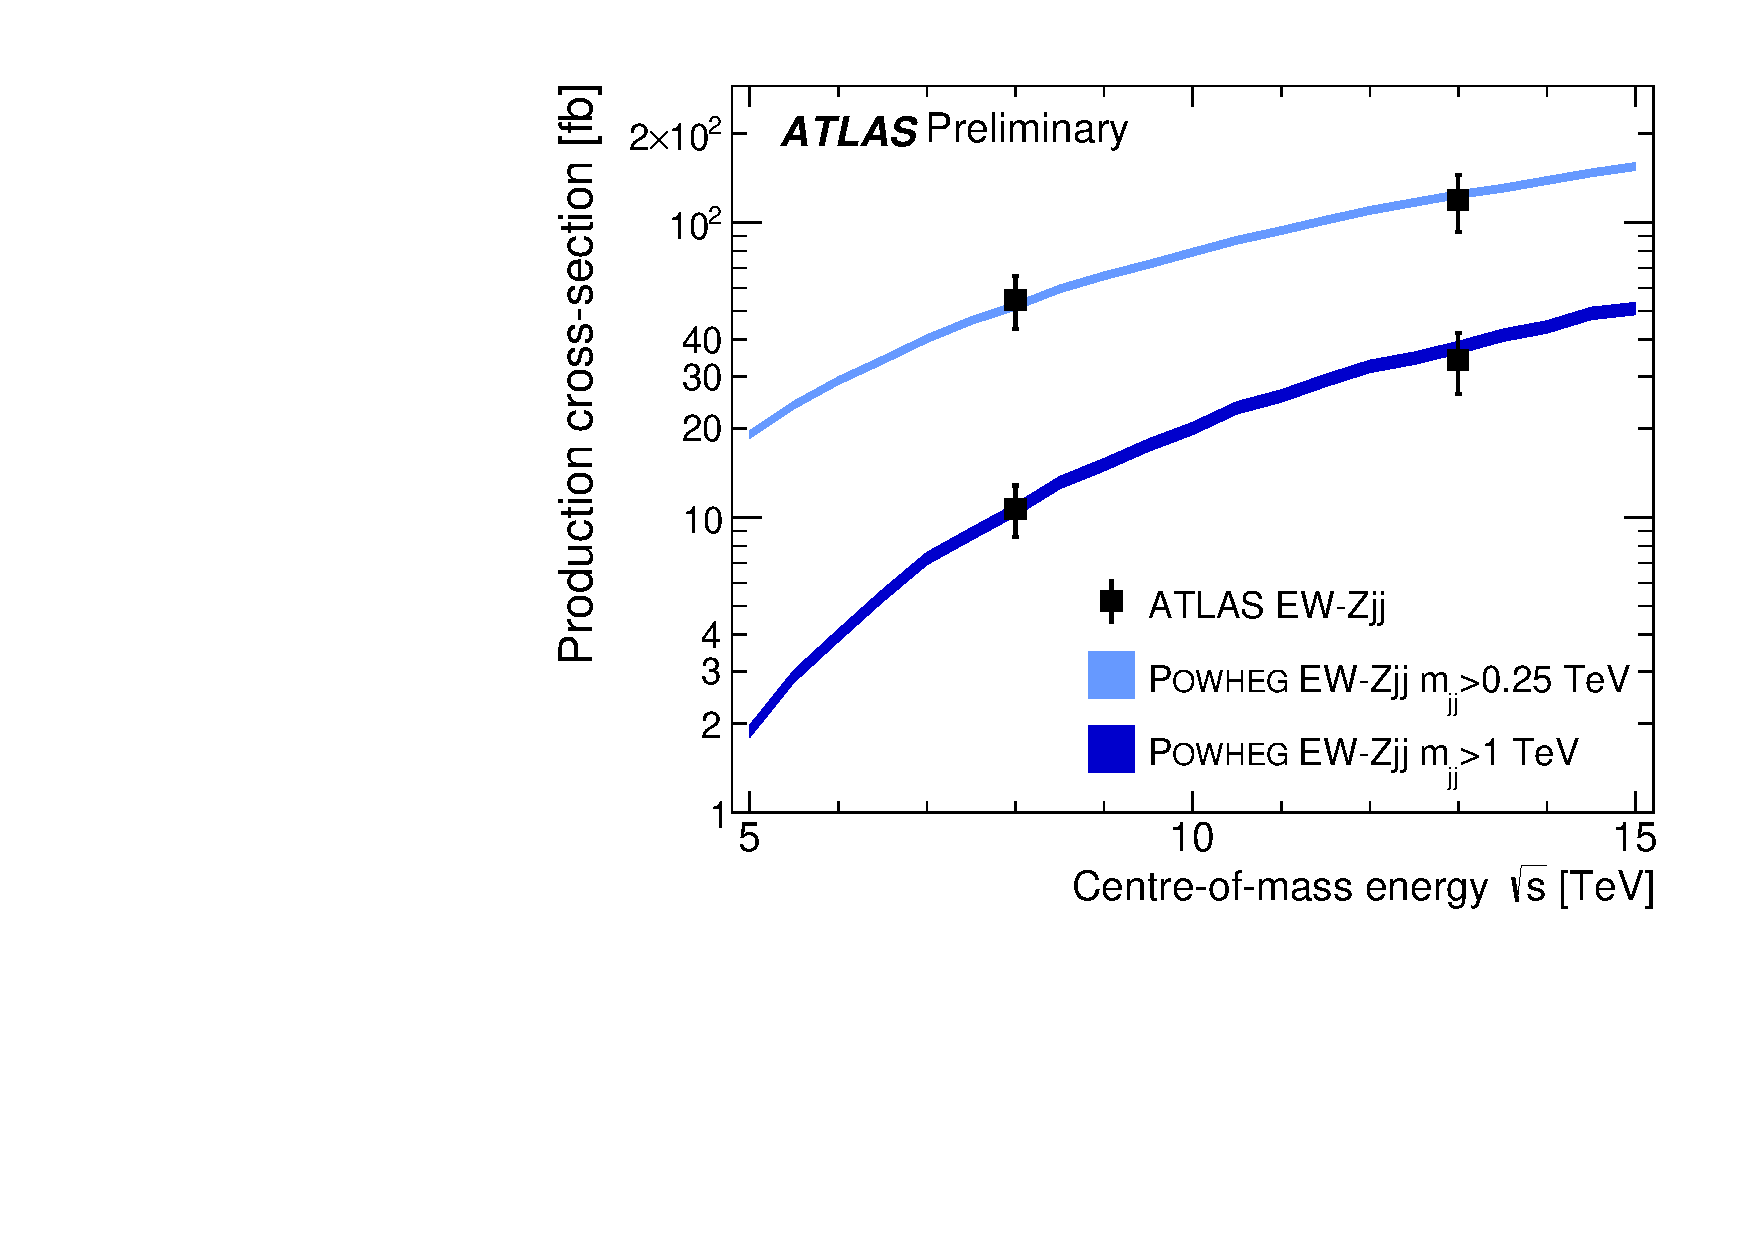
\includegraphics[width=.57\textwidth]{STDM-2016-09/fig_06.pdf}
  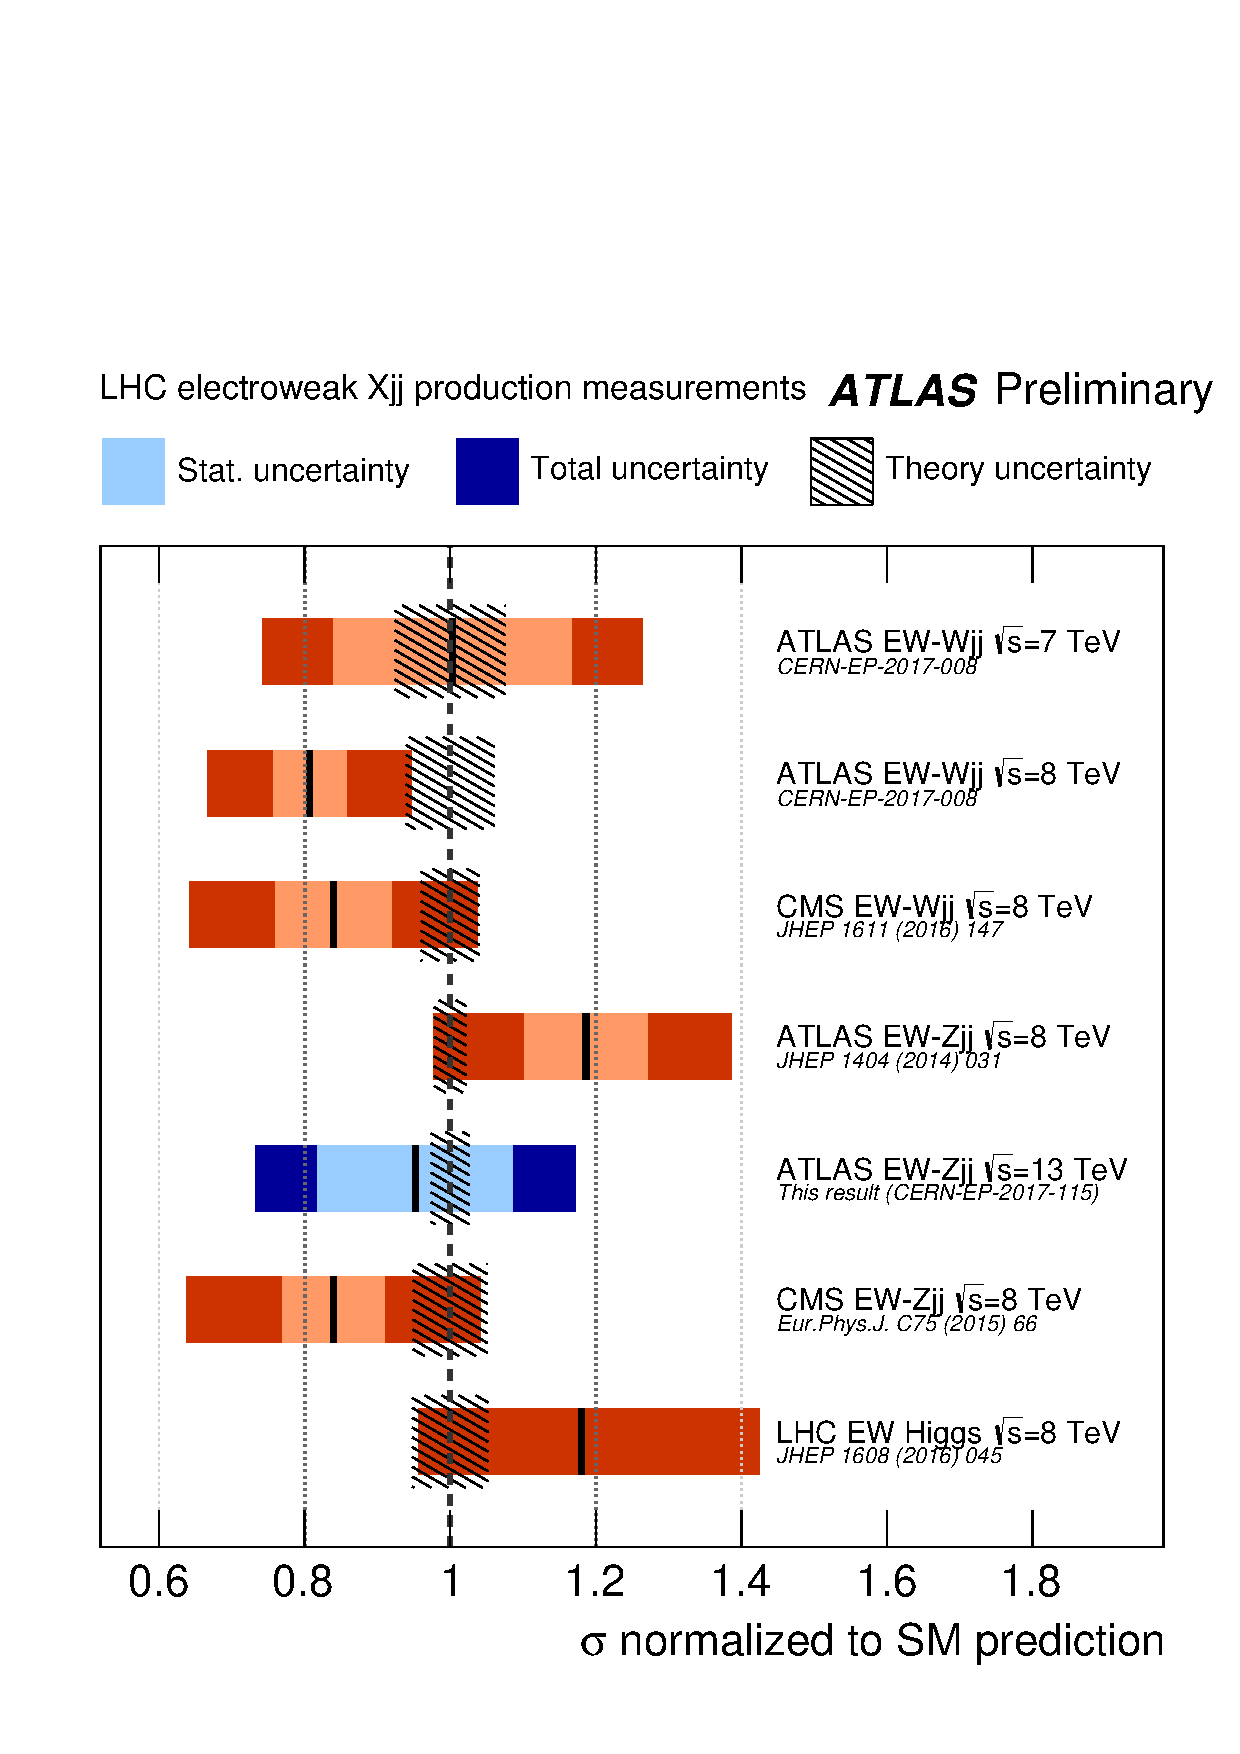
\includegraphics[width=.42\textwidth]{STDM-2016-09/fig_09.pdf}
  \caption{Left: \zjj measurement vs center-of-mass energy. Right: summary of electroweak \wjj and \zjj
measurements at ATLAS and CMS.}
  \label{zjj-wjj-summary-results}
\end{figure}


\bibliographystyle{JHEP}
\bibliography{my-bib-database}

\end{document}
